% Szkielet dla pracy pisanej w języku angielskim.

\documentclass[polish,a4paper,twoside]{ppfcmthesis}

\usepackage[utf8]{inputenc}
\usepackage[OT4]{fontenc}
\usepackage{listings}
\usepackage{amsfonts}
\usepackage{amsmath}
\usepackage{float}




\author{Jakub Bręk}                              % Your name comes here
\title{Programowanie wizualne urządzeń mobilnych}        % Note how we protect the final title phrase from breaking
\ppsupervisor{Rafał Różycki, ~Dr.~Hab.} % Your supervisor comes here.
\ppyear{2014}                                         % Year of final submission (not graduation!)

\begin{document}

% Front matter starts here
\frontmatter\pagestyle{empty}%
\maketitle\cleardoublepage%

\pagebreak

% Blank info page for "karta dyplomowa"
\thispagestyle{empty}\vspace*{\fill}%
\begin{center}Tutaj przychodzi karta pracy dyplomowej;\\oryginał wstawiamy do wersji dla archiwum PP, w pozostałych kopiach wstawiamy ksero.\end{center}%
\vfill\cleardoublepage%

\pagebreak

% Table of contents.
\pagenumbering{Roman}\pagestyle{ppfcmthesis}%
\tableofcontents* \cleardoublepage%

% Main content of your thesis starts here.
\mainmatter%
\chapter{Wprowadzenie}
\label{c1}

\section{Programowanie}
\label{c11}

Programowanie jest to między innymi proces tworzenia aplikacji. Jest ono głównie kojarzone z wielkimi ilościami kodu napisanego przez programistów. W większości przypadków tak jest. Jednak sposób pisania kodu może się różnić. Można wydzielić programowanie od bardzo niskiego poziomu do wysokiego poziomu. Przy językach niskiego poziomu, np. Assembler operowanie odbywa się na rejestrach procesora. Operacje są bardzo szybkie, jednak napisanie czegoś bardziej skomplikowanego zajęłoby ogromną ilość lini kodu oraz czasu. Następnie istnieją języki wyższego poziomu, którego składnia ułatwia zrozumienie kodu programu przez osoby, które mają z tym kodem styczność.

Aby jeszcze lepiej zrozumieć pisany kod powstała jeszcze jedna warstwa abstrakcji, gdzie tak naprawdę nie jest wymagana od programistów ani jedna linijka kodu. Jest to programowanie wizualne. Główne źródło tworzonego oprogramowania stanowią bloki graficzne i połączenia między nimi.


\subsection{Programowanie wizualne}
\label{c111}
Programowanie wizualne jest to programowanie, które pozwala użytkownikowi tworzyć programy poprzez manipulację elementów graficznie, inaczej niż w większości przypadków przy użyciu edytorów tekstowych. Prawie wszystkie akcje, które możliwe do osiągnięcia mogą zostać zrealizowane tylko za pomocą myszki.

Jednym z narzędzi, które pozwala tworzyć aplikacje wizualnie jest App Inventor. Za pomocą powyższego programu istnieje możliwość tworzenia aplikacji na system operacyjny android. Są to głównie telefony i tablety. App Inventor jest aplikacją internetową, dostępną z poziomu przeglądarki. Nie potrzebujemy dodatkowego środowiska do tworzenia programów. App inventor jest aplikacją stworzoną przez Google, a aktualnie utrzymywaną przez uniwersytet Massachusetts Institute of Technology (MIT). Wszystkie nowe osoby, które chciałyby zacząć programować i tworzyć oprogramowanie na system operacyjny Android mogą zacząć od App Inventora. Tworzenie aplikacji jest intuicyjne dzięki graficznemu interfejsowi, który umożliwia użytkownikowi akcje typu "przeciągnij i upuść" na interesujących go obiektach.\cite{wiki:appinventor} Są to proste czynności, które nie wymagają głębokiej wiedzy informatycznej. Osoby, które nigdy nie miały do czynienia z programowaniem, nie będą miały większych kłopotów z napisaniem aplikacji.

\subsection{Programowanie natywne}
\label{c112}

Programowanie natywne jest to programowanie na daną platformę, a więc napisane oprogramowanie będzie na niej działać bez dodatkowych programów. W przypadku systemu Android jest to język Java. Jest to język obiektowy wysokiego poziomu. Po napisanu programu, kod jest kompilowany do kodu bajtowego, którym zajmuje się maszyna wirtualna javy (JVM). Ładuje pliki do pamięci, a następnie uruchamia zawarty w nich kod. Jednak Android nie posiada JVM. Zamiast JVM, Google wyposażył Android w maszynę Dalvik'a. Dalvik jest to maszyna wirtualna, przystosowana specjalnie do urządzeń mobilnych, gdzie szczególną uwagę należy zwrócić na małe zasoby pamięci, energii i niewielką prędkość procesorów. Kod bajtowy stworzony przez kompilator nie jest w 100\% kompatybilny z kodem bajtowym Javy. Nie można tutaj korzystać z bardziej zaawansowanych cech jakimi są Class Loadery czy Java Reflection API. \cite{gphone:dalvik}

\section{Cel i zakres pracy magisterskiej}
\label{c12}

Celem pracy magisterskiej jest porównanie tworzenia aplikacji na platformę android przy pisaniu aplikacji w języku Java, oraz przy wykorzystaniu narzędzia oferowanego online - App Inventor. Praca zawiera porównanie tworzenia oprogramowania z różnych perespektyw, między innymi takich jak:
\begin{itemize}
\item Czas potrzebny na stworzenie aplikacji
\item Możliwości jakie daje nam App Inventor, jakich rzeczy tam brakuje, a co można użyć
\item Łatwość stworzenia aplikacji
\item Porównanie takich samych aplikacji pod względem zużycia procesora oraz pamięci
\item Porównanie wydajności tych samych algorytmów pod względem czasu
\item Jak wygląda stworzenie bardziej zaawansowanej aplikacji korzystającej z wielu funkcji telefonu
\item Czy jakieś dodatkowe narzędzia są potrzebne do tworzenia aplikacji
\end{itemize}

Dzięki takiemu porównaniu powstanie czystszy obraz na narzędzie jakim jest App Inventor. Młodsze osoby zainteresowane programowaniem łatwiej będą mogły się zdecydować, w którą stronę pójść. Czy warto w ogóle zawracać sobie głowę App Inventorem, czy odrazu uczyć się Javy i mieć dostęp do wszystkch funkcji Androida. Dodatkowo nauczyciele informatyki będą mogli rozważyć naukę podstaw programowania poprzez tworzenie aplikacji na system Android.

W pracy zostały również przedstawione wady oraz zalety pisania oprogramowania przy wykorzystaniu App Inventora. Programowanie wizualne, mimo że wydaje się łatwiejsze niesie ze sobą również pewne niedogodności. Pewnych rzeczy prawdopodobnie nie da się zrealizować, a pewne są możliwe do zrealizowania w wiele prostszy sposób.


\subsection{Struktura pracy magisterskiej}

W rozdziale \Ref{c2} przedstawiono podstawowe pojęcia, które zostały użyte przy pisaniu pracy magisterskiej. Terminy te zostały wyjaśnione, aby bez problemu zrozumieć bardziej skomplikowane zagadnienia.

W rozdziale \Ref{c2} zawarto teorię dotyczącą App Inventora.

W rozdziale \Ref{c4} pokazano zastosowane podejście do rozwiązania problemu.

W rozdziale \Ref{c5} przedstawiono wyniki uzyskanep podczas pisania pracy magisterskiej.












\chapter{Podstawowe pojęcia}
\label{c2}

W danym rozdziale zostaną zawarte podstawowe pojęcia i mechanizmy używane przez aplikację App Inventor. Ideą tutaj jest przypomnienie oraz przypliżenie ważnych terminów informatycznych.

\section{App Inventor}
\label{c21}

W grudniu 2013 roku został wydany App Inventor w wersji drugiej. Starsza wersja została nazwana jako Classic. Oba narzędzia są bardzo podobne jednak projekty stworzone w starszej wersji nie mogą zostać zaimportowane do nowszej. W danej pracy magisterskiej skupienie zostało na nowej wersji App Inventora.

App Inventor jest to system, który pozwala na tworzenie aplikacji używając jedynie przeglądarki internetowej. Jest to aplikacja internetowa, umożliwiająca zrobienie programu, przez użytkowników mających bardzo małe pojęcie o programowaniu. 

Potencjał aplikacji jest bardzo duży. Można to zauważyć patrząc na ilość aktywnych użytkowników. W maju 2014 roku, liczba aktywnych użytkowników wynosiła 87tys. tygodniowo. Ilość zarejestrowanych to 1,9mln w 195 krajach. Użytkownicy ci stworzyli razem 4,7mln projektów.\cite{article:appinventor1}

\section{Główne komponenty}
\label{c22}

App Inventor celowo ułatwia programowanie poprzez wizualizację tworzonych komponentów i intuicyjny interfejs. App Inventor składa się z 3 głównych komponentów jakimi są:
\begin{itemize}
\item App Inventor Designer
\item App Inventor Blocks Editor
\item Android Device Emulator
\end{itemize}

\subsection{App Inventor Designer}
\label{c221}

Jednym z głównych widoków jakie można używać jest widok Designera. Projektowanie interfejsu użytkownika polega na przeciąganiu komponentów z dostępnej palety, wliczając w to także niewidoczne komponenty takie jak sensory. W tym widoku można również zmieniać właściwości obiektów, które zostały stworzone. Między innymi istnieje możliwość zmiany położenia, wielkości, układu (pionowy, poziomy).

Designer jest zaprojektowany jako zwykła aplikacja internetowa. Tak więc uruchamia się go, jak zwykłą stronę internetową wpisując jej adres www.

\begin{figure}[th] 
\centering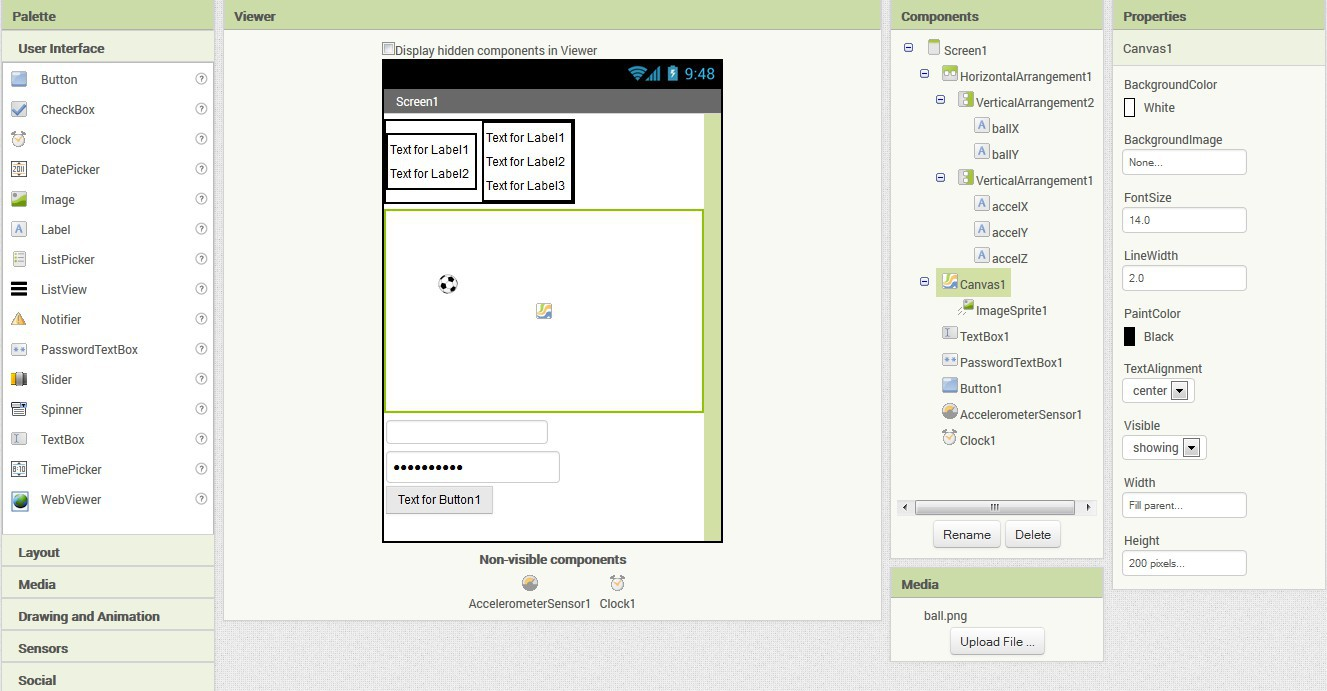
\includegraphics[width=10cm]{figures/designer}
\caption{App Inventor Designer}
\end{figure}

\subsection{App Inventor Blocks Editor}
\label{c222}

Drugim widokiem jest Blocks Editor. Zachowanie aplikacji zostaje tutaj zaprogramowane poprzez połączenie odpowiednich bloków. Istnieje możliwość korzystania z bardziej generalnych komponentów, a także z bardziej specyficznych. Dla każdego komponentu, który został stworzony w interfejsie graficznym (Designerze) są dostępne bloki mówiące, co tak naprawdę jest możliwe do zrobienia. Wygląda to w ten sposób, że komponenty są przciągane z dostępnej palety medotą "przeciągnij i upuść", a następnie łączone jak puzzle.

Ta część aplikacji normalnie reprezentowana jest przez kod napisany przez programistę. Więc napisanie zachowania aplikacji odbywa się poprzez łączenie puzzli, bez znajomości języka Java.

\begin{figure}[th] 
\centering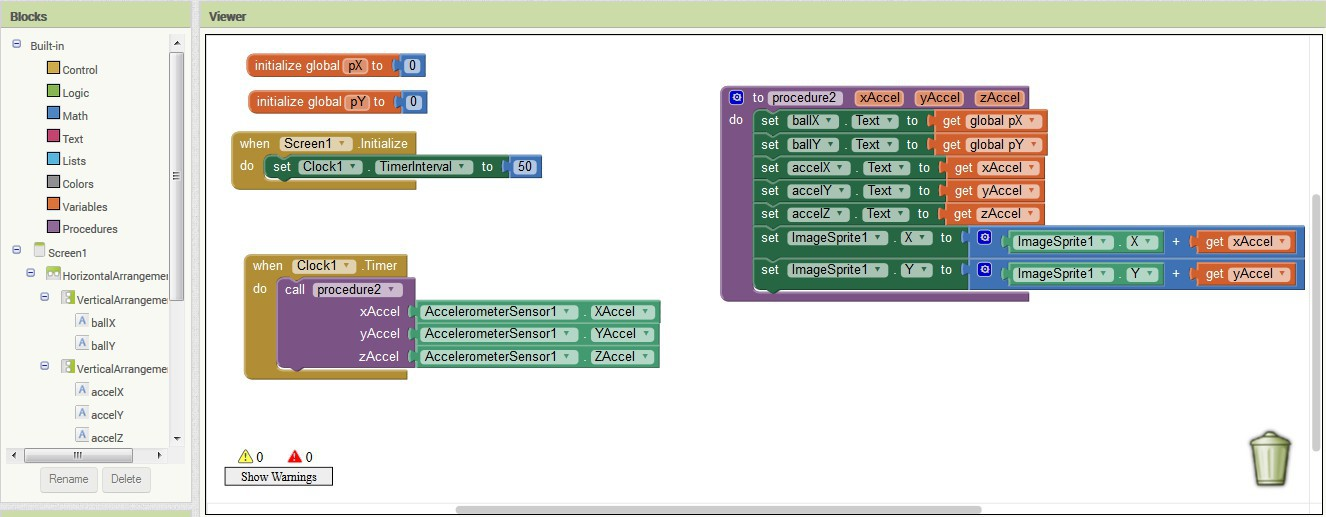
\includegraphics[width=10cm]{figures/editor}
\caption{App Inventor Blocks Editor}
\end{figure}

\subsection{Android Device Emulator}
\label{c223}

Android Device Emulator jest to emulator telefonu lub tabletu. Jest to wirtualna wersja smartphonu, w której znajdują się obsługa dotyku ekranu, przyciski systemowe oraz typowe funkcje.

Zmiany, które zostają wprowadzone, natychmiast reflektują na działanie aplikacji. Nie ma potrzeby jakiejkolwiek kompilacji i uruchamiania aplikacji od nowa. Jeżeli aplikacja zostanie uruchomiana, kompilacja zmienionych fragmentów oraz zainstalowanie ich na emulatorze dzieje się w czasie rzeczywistym. Jest to bardzo wygodna opcja budowania aplikacji i testowania jej. Zmiany, które zrobimy są od razu widoczne na ekranie.

\begin{figure}[th] 
\centering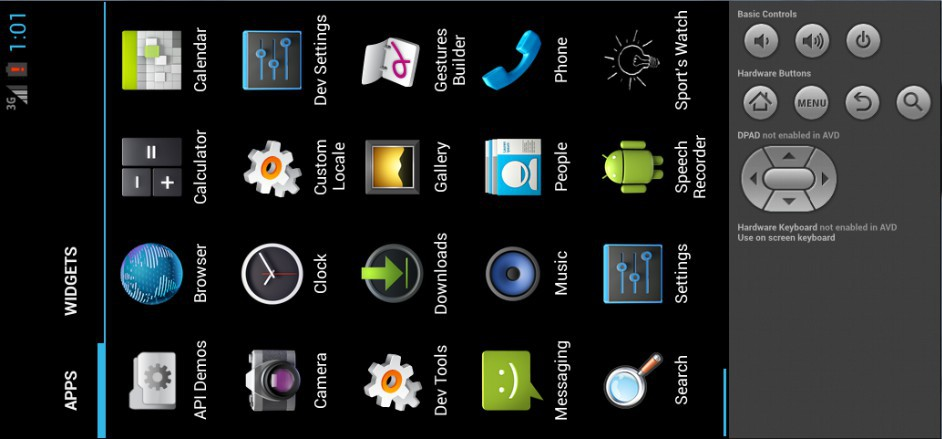
\includegraphics[width=10cm]{figures/emulator}
\caption{Android Device Emulator}
\end{figure}

\section{Pozostałe istotne komponenty}

W danym rozdziale zostały zawarte pozostałe komponenty, które zostały użyte podczas pisania pracy. Związane są one zarówno z App Inventorem, jak i z aplikacjami napisanymi w Javie.

\subsection{Android SDK}

Android SDK - jest to zestaw narzędzi programistycznych, które są oferowane dla programistów, chcących tworzyć aplikacje na platformę Android. Jest on modularny, poprzez SDK Managera, możemy zainstalować, tylko te komponenty, które nas interesują. 

\subsection{SDK Tools}

Android SDK dzieli się na dwie części SDK Tools oraz Platform Tools. Najważniejsze narzędzia wchodzące w skład pierwszej części to:
\begin{itemize}
\item AVD Manager - odpowiedzialny za zarządzanie wirtualnymi urządzeniami z systemem operacyjnym android. Jest to najłatwiejsza i najwygodniejsza opcja stworzenia nowego wirtualnego urządzenia i odpowiedniego sparametryzowania go.
\item SDK Manager - wspomniany wyżej, odpowiedzialny za instalację modułów, które nas interesują
\item Emulator - emualtor systemu android, stworzony przez AVD Managera
\item Dalvik Debug Monitor (DDMS) \label{ddms}- jest to narzędzie pomocne w debugowaniu aplikacji. Dostarcza on takich funkcji jak przekierowanie portów, przechwyt obrazu na urządzeniu, informacje o wątkach, stosie, a także o metodach, które są uruchomione jeżeli włączymy ich profilowanie.
\end{itemize}

\subsection{Platform Tools}

\begin{itemize}
\item Android Debug Bridge \label{adb}- narzędzie pozwalające na komunikację z podłączonym urządzeniem. Jest także używany do instalacji i uruchamiania aplikacji. Składa się z 2 części, klienta i serwera, które komunikują się ze sobą.
\end{itemize}

\subsection{Apktool}

Jest to narzędzie do tak zwanej inżynierii odwrotnej (\english{Reverse engineering}). Umożliwia ono dekodowanie programu do prawie oryginalnej formy. Następnie, po dokonaniu pewnych modyfikacji umożliwia ono zbudowanie aplikacji z powrotem do wyjściowej formy.\cite{doc:apktool}

\subsection{Keystore}

Jest to repozytorium przechowujące certyfikaty bezpieczeństwa. Do zarządzania certyfikatami istnieje narzędzie o nazwie keytool. Umożliwia ono użytkownikom zarządzanie prywatnymi/publicznymi kluczami, certyfikatami jak i podpisem elektornicznym.\cite{doc:keytool}

\subsection{Jarsigner}

System android wymaga, aby aplikacje na nim instalowane były cyfrowo podpisane. Dzięki temu system może zweryfikować autora aplikacji. Podpisywanie aplikacji dzielimy na 2 sposoby: tryb debugowania (\english{Debug mode})oraz tryb wydania (\english{Release mode}). Przy korzystaniu ze zintegrowanego środowiska programistycznego zwykle aplikacja zostaje cyfrowo podpisana automatycznie, podczas instalacji jej na telefonie. Jarsigner umożliwia popisanie aplikacji manualnie, korzystając z lini poleceń.

\subsection{Zużycie procesora}

Czas pracy procesora jest to czas, w którym procesor (\english{CPU}) został użyty to przetwarzania zadanych instrukcji, w przeciwieństwie do oczekiwania na wejście/wyjście lub przejścia w stan oczekiwania (\english{Idle mode}). Zużycie procesora natomiast mierzone jest w procentach jako całkowitej wydajności procesora. Główne zastosowanie to określenie ogólnej zajętości systemu. Wysokie zużycie procesora oznacza zbyt małą moc procesora, lub zbyt wygórowane oczekiwania użytkownika.


\section{Ważne koncepcje i pojęcia dotyczące App Inventora}

Istnieje kilka pojęć, które są warte uwagi. Zostały one zawarte w tym rozdziale.

\subsection{Publikacja aplikacji na Google Play}

Aplikacje zbudowane za pomocą App Inventora mogą zostać przesłane do marketu Google Play. Każda aplikacja, która ma zostać opublikowana musi posiadać wersję kodu (\english{VersionCode}) oraz nazwę wersji (\english{VersionName}). Te parametry można ustawić we właściwościach głównego komponentu\cite{doc:concepts}. Wersja kodu jest to całkowita wartość, która nie jest widoczna dla użytkowników w Google Play. Potrzebna jest do sprawdzenia czy aplikacja została aktualizowana lub dezaktualizowana do poprzedniej wersji. Nazwa wersji może być dowolna jednak wg konwencji powinna to być liczba zmiennoprzecinkowa. Domyślnie posiada wartość 1.0. Jest ona zwiększana o 0.1 lub 1 dla małej i dużej zmiany.

Skończony projekt możemy wyeksportować do pliku .apk, który jest automatycznie cyfrowo podpisany kluczem prywatnym powiązanym z naszym kontem. Kiedy tworzymy nową wersję ten sam klucz jest używany do podpisu. Kiedy urządzenie z system android posiada zainstalowaną aplikację, zapamiętuje on klucz który został użyty do podpisu. Aby zainstalować wyższą wersję aplikacji ten sam klucz musi zostać użyty do podpisu.

Repozytorium keystore, w którym znajduje się klucz domyślnie jest stworzone na serwerze, więc nie trzeba się tym martwić. Istnieje również opcja eksportu i importu repozytorium. Jest ona przydatna przy przenoszeniu projektu na inny serwer.

\subsection{Paleta z dostępnymi komponentami}

\begin{itemize}

\item \textbf{User Interface} - w większości widoczne komponenty, które są związane z interfejsem użytkownika.
\begin{itemize}
\item Button - przycisk.
\item CheckBox - pole wyboru.
\item DatePicker - komponent dający możliwość wyboru daty.
\item Image - komponent umożliwiający wyświetlenie przesłanego zdjęcia.
\item Label - etykieta, na której zwykle wyświetlany jest kawałek tekstu.
\item ListPicker - komponent, który po kliknięciu wyświetla listę, z której użytkownik może wybrać wartość. Daje on także możliwość automatycznego osadzenia wyszukiwarki na liście.
\item ListView - komponent, który pozwala na osadzenie i wyświetlenie listy elemenentów
\item Notifier - komponent wyświetlający powiadomienia, a także umożliwiający logowanie na 3 poziomach (Error, Warn, Info).
\item TextBox - komponent umożliwiający wpisywanie tekstu.
\item PasswordTextBox - taki sam komponent jak TextBox jednak wpisywany tekst nie jest widoczny dla użytkownika.
\item Slider - jest to pasek postępu, który dodatkowo umożliwia użytkownikowi przeciąganie.
\item Spinner - element wyświetlający pop-up z listą elementów do wyboru.
\item TimePicker - element pozwalający na wybór czasu.
\item WebViewer - komponenet umożliwiający umieszczenie dowolnej strony internetowej w aplikaji.
\end{itemize}

\item \textbf{Layout} - Komponenty odpowiedzialne za rozmieszczenie pozostałych komponentów. Są to kontenery, w które mogą zostać umieszczane inne widoczne komponenty.
\begin{itemize}
\item HorizontalArrangement - elementy umieszczone w tym kontenerze są układanej od lewej do prawej.
\item VerticalArrangement - odwrotne działanie do poprzedniego komponentu - elementu są umieszczany od góry do dołu.
\item TableArrangement - element umożliwiający ustawienie elementów postaci tabularnej
\end{itemize}


\item \textbf{Media} - Komponenty związane głównie z dźwiękiem oraz kamerą.
\begin{itemize}
\item Camcorder - komponent umożliwiający nagrywanie filmów. Istnieje możliwość nadania nazwy pliku zawierającego nagranie.
\item Camera - komponent umożliwiający robienie zdjęć i zapisywanie ich.
\item ImagePicker - komponent uruchamiający galerię zdjęć zawartą na telefonie i dający możliwość wyboru zdjęciu. Zdjęcie po wybraniu jest kopiowane na kartę SD (maksymalna ilość zdjęć to 10). Następnie możemy z danego zdjęcia skorzystać w aplikacji i je wyświetlić.
\item Player - komponent odtwarząjący muzykę, a także odpowiedzialny za wywołanie wibracji w telefonie.
\item Sound - komponent odtwarzający dźwięki, w porównaniu do poprzedniego, dźwięki powinny mieć krótki czas trwania, podczas gdy muzyka może trwać długo.
\item SoundRecorder - komponent nagrywający dźwięk
\item SpeechRecognizer - komponent umożliwiający rozpoznanie mowy i stworzenie z niej tekstu
\item TextToSpeech - komponent o odwrotnym działaniu do poprzedniego, zamieniający tekst na mowę. Wsparcie dla języków: czeski, hiszpański, niemiecki, francuski, duński, włoski, polski, angielski.
\item VideoPlayer - komponent umożliwiający odtwarzanie filmu podczas działającej aplikacji. Pliki wideo muszą mieć poniżej 1MB, dodatkowo rozmiar całkowitej aplikacji wynosi maksymalnie 5MB.
\item YandexTranslate - komponent umożliwiający tłumaczenie tekstu pomiędzy językami. Korzysta on z serwisu o nazwie Yandex - https://translate.yandex.com. dodatkowo urządzenie musi być podłączone do internetu. 
\end{itemize}


\item \textbf{Drawing and Animation} Komponenty umożliwiające rysowanie oraz animacje.
\begin{itemize}
\item Canvas - płótno, na którym możemy rysować dwuwymiarowe obrazki (\english{Sprite}). Obrazki te mogą się na płótnie poruszać. Każda lokalizacja na płótnie jest specyfikowana za pomocą współrzędnych X,Y.
\item ImageSprite - obrazek, który możemy umieścić na płótnie i który może reagować na dotyk, przeciąganie
\item Ball - jest to ImageSprite, który ma ustawiony obrazek jako koło o określanym kolorze.
\end{itemize}

\item \textbf{Sensors} Niektóre z sensorów, dostępnych na telefonie. Wszystkie z tych komponentów są niewidoczne.
\begin{itemize}
\item AccelerometerSenser - akcelerometr, komponent, który umożliwia wykrycie trzęsienia telefonem, a daje wartości, odpowiadające aktualnemu wychyleniu telefonu.
\item BarcodeScanner - komponent umożliwiający skanowanie kodów kreskowych, jednak musimy posiadać dodatkowo aplikację do tego zainstalowaną już na telefonie.
\item Clock - Zegar oraz czasomierz
\item LocationSensor - komponent dostarczający informacje o położeniu gdzie się znajdujemy, czyli szerokość i długość geograficzną. Informacje te mogą nie być odrazu dostępne i musimy na nie poczekać.
\item NearField - komponent dostarczający możliwośći NFC. Dotychczas komponent ten umożliwia czytanie i wysyłanie tagów tekstowych.
\item OrientationSensor - żyroskop - komponent dostarczający informację o urządzeniu w 3 wymiarach.
\end{itemize}

\item \textbf{Social} - komponenty związane z kontaktami, e-mailami i serwisami społecznościowymi.
\begin{itemize}
\item ContactPicker - przycisk, który po naciśnięciu wyświetla listę kontaktów do wyboru. Gdy użytkownik dokona wyboru ma dostęp do następujących danych: nazwa kontaktu, e-maile, telefony, zdjęcie kontaktu.
\item EmailPicker - textBox z pomocą dla użytkownika. Pomoc ta polega na wyświetleniu listy, która zawiera emaile pasujące do wpisywanego tekstu.
\item PhoneCall - komponent umożliwiający uruchomienie dzownienia do osoby, którą wcześniej ustawimy jako właściwość komponentu.
\item PhoneNumberPicker - przycisk o podobnym działaniu do komponentu ContactPicker.
\item Sharing - niewidoczny komponent, który umożliwia udostępnienie wiadomości lub pliku innym aplikacjom
\item Texting - komponent odpowiedzialny za zarządzanie wiadomościami. Jeżeli aplikacja działa w tle, zdarzenie przyjścia wiadomości również będzie uruchomione. Nawet jeżeli aplikacja nie jest uruchomiona pojawi się powiadomienie o przyjściu wiadomości, po kliknięciu w nie uruchomi się aplikacja
\item Twitter - komponent umożliwiający komunikację z serwisem internetowym Twitter. Jeżeli użytkownik zostanie pozytywnie zautentykowany i zautoryzowany, pojawia się wiele możliwości, min. szukanie tweetów, wysyłanie tweetów, wiadomości, obrazków.
\end{itemize}

\item \textbf{Storage} - komponenty odpowiedzialne za przechowywanie danych.
\begin{itemize}
\item File - niewidoczny komponent umożliwiający zapis i odczyt pliku. Domyślne ustawienia zapisują pliki do prywatnego katalogu App Inventora, jednak istnieje możliwość ustawienia innej ścieżki
\item FusiontablesControl - komponent, który komunikuje się z serwisem internetowym dostarczonym przez Google o nazwie Fusion Tables. Tabele te umożliwiają wizualizację, udostępnienie, zapis danych. Komponent ten daj możliwość dostępu do tych danych a także jej edycji.
\item TinyDB - baza danych dla aplikacji. Jest to odpowiednik klasy Javy - SharedPreferences. Można sobie ją wyobrazić jako mapę - klucz/wartość.
\item TinyWebDB - niewidoczny komponent, komunikujący się z internetową bazą danych.
\end{itemize}

\item \textbf{Connectivity} - komponenty umożliwiające komunikację i uruchmianie innych apliakcji.
\begin{itemize}
\item ActivityStarter - komponent do uruchamiania zewnętrznych Activity. Przez Activiy są rozumiane: inne aplikacji napisane w App Inventorze, kamera, wyszukiwarka internetowa, otwieranie strony internetowej, otwieranie aplikacji mapy w zadanej lokalizacji.
\item BluetoothClient - komponent blutetooth klienta.
\item BluetoothServer - komponent bluetooth serwera.
\item Web - komponenet umożliwiający wysyłanie żądań typu REST do serwera. Dostarcza od funkcje: GET, POST, PUT, DELETE.
\end{itemize}

\item \textbf{LEGO MINDSTORMS} - komponenty dostarczające kontrolę nad robotami poprzez bluetooth. W danej pracy magisterskiej zostały pominięte, ze względu na brak powyższych robotów.
\end{itemize}







\chapter{Teoria}
\label{c3}

\section{Wstęp}
\label{c31}

W niniejszym rozdziale zawarto opis architektury oraz główne komponenty wykorzystywane przez App Inventora. Pomoże to zrozumieć zalety oraz wady powyższego narzędzia.

\section{Architektura}
\label{c32}

Każda aplikacja ma swoją wewnętrzną strukturę, którą trzeba dokładnie zrozumieć, aby tworzyć efektywne oprogramowanie. Architektura aplikacji składa się głównie z 2 części: komponenty oraz ich zachowanie. Można z pewnym dystansem przyjąć, że za komponenty odpowiada widok Designera, a za zachowanie komponentów widok edytora.

\begin{figure}[th] 
\centering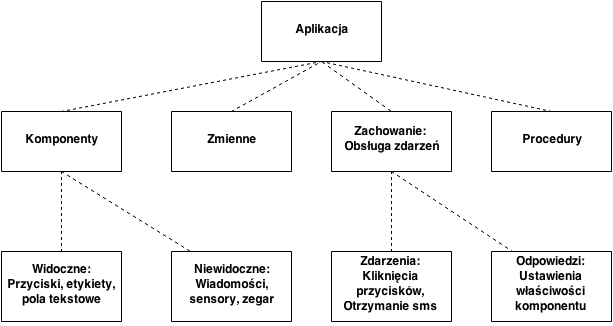
\includegraphics[width=12cm]{figures/architektura}
\caption{Architektura aplikacji stworzonej przez App Inventora\cite{appinventor:architektura}}
\end{figure}

\subsection{Komponenty}
\label{c321}

Komponenty można podzielić na 2 rodzaje: widoczne oraz niewidoczne. 
\begin{itemize}
\item Widoczne użytkownik widzi gołym okiem. Należą do nich przyciski, etykiety, pola tekstowe. Definiują one interfejs użytkownika.
\item Niewidocznych komponentów, jak sama nazwa wskazuje, użytkownik nie widzi. Nie są one częścią interfejsu. Dostarczają one dostępu do wbudowanych funkcjonalności telefonu. Są to różne sensory np. akcelerometr, moduł gps, komponent zamiany tekstu na mowę itp.
\end{itemize}

Oba rodzaje komponentów posiadają zbiór swoich właściwości. Właściwości danego komponentu są to informacje jakie komponent posiada. Etykieta posiada między innymi rodzaj, wielkość, dekorację, kolor czcionki, wielkość, widoczność etykiety. Użytkownik nie widzi danych właściwości, obserwuje on rezultat konkretnych ustawień na ekranie urządzenia.

\subsection{Zachowanie aplikacji}
\label{c322}
Zrozumienie zasady tworzenia komponentów i ich właściwości jest proste. Nazwy komponentów są intuicyjne, więc nie powinno być problemu z odnalezieniem tego, który interesuje programistę. Z drugiej strony zachowanie komponentów może okazać się bardziej skomplikowane. Mimo wszystko App Inventor stara się wizualizować bloki opisujące zachowanie w jak najprostszej formie.

Kiedy zaczynano pisać aplikacje, można było je porównać do recept, gdzie ciąg zdarzeń ukazany jest jako liniowa sekwencja instrukcji. Typowa aplikacja może uruchomić transakcję w banku, dokonać pewnych obliczeń, zmodyfikować stan konta i na koniec wyświetlić nowe saldo.\cite{appinventor:architektura}

W dzisiejszych czasach większość aplikacji nie wpasowuje się w powyższy schemat. Zamiast wykonywać ciąg instrukcji w odpowiedniej kolejności, reagują na zdarzenia, które są inicjowane przez użytkownika danej aplikacji. Jednym z przykładów jest kliknięcie przycisku lub trzęsienie telefonem, który jest zaprogramowany tak, aby na każdy bodziec móc umieć odpowiedzieć. Wiele zdarzeń jest inicjowanych przez użytkownika, ale są też wyjątki. Aplikacja może reagować na zdarzenia, które w nie wymagają interakcji z użytkownikiem. Często są to niewidoczne komponenty umieszczone w Designerze. Poniższy rysunek prezentuje aplikację otoczoną wieloma zdarzeniami.

\begin{figure}[th] 
\centering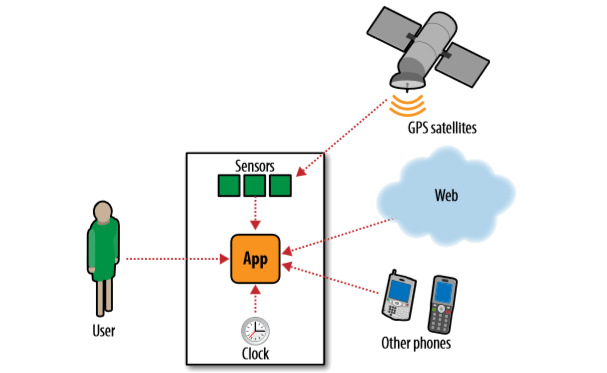
\includegraphics[width=10cm]{figures/events}
\caption{Aplikacja reagująca na zdarzenia zewnętrzne i wewnętrzne\cite{appinventor:architektura}}
\end{figure}

Jednym z powodów dlaczego App Inventor jest tak intuicyjny jest zastosowanie prostej koncepcji nazywania zdarzeń. Zdefiniowanie zdarzenia polega na przeciągnięciu go z palety na główny ekran, a następnie napisanie konkretnego zachowania. Przykładem takiego zdarzenia jest obsługa akcelerometru. Po zatrzęsieniu telefonem, pojawia się tekst \emph{Shaking!}.

\begin{figure}[th] 
\centering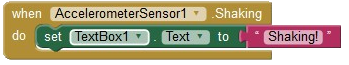
\includegraphics[width=10cm]{figures/shakingEvent}
\caption{Obsługa zdarzenia trzęsienia telefonem}
\end{figure}

Zdarzenia można podzielić w zależności od jego typu:
\begin{itemize}
\item Zainicjowane przez użytkownika - najbardziej popularny typ zdarzenia - głównie jest to obsługa zdarzeń dotyku ekranu.
\item Inicjalizujące - są wykonywane, gdy dany komponent jest tworzony.
\item Czasowe - są uruchamiane, co pewien interwał czasowy.
\item Animacje - są zależne od obiektów (spritów) które zostały stworzone. Mogą zostać uruchomione gdy obiekty ze sobą kolidują, wylatują poza ekran.
\item Zewnętrzne - są uruchamiane gdy urządzenie odbierze jakiś sygnał zewnętrzny typu, odczyt pozycji urządzenia z satelity, reakcja na przychodzący sms.
\end{itemize}

Programowanie aplikacji odbywa się poprzez zdefiniowanie interfejsu, a następnie napisanie zachowania danej aplikacji, dla różnych zdarzeń, które mogą wystąpić. Inaczej mówiąc, komponenty tworzone są najpierw w Designerze i tam przypisywane są do nich właściwości. Programista po otrzymaniu interesującego go wyglądu może przystąpić do opisu zdarzeń.

\section{Debugowanie aplikacji}
\label{c33}

Najłatwiejszy sposób instalacji i testowania aplikacji odbywa się przez wifi. Musimy pobrać dodatkową aplikację na urządzenie z systemem Android. Następnie na stronie App Inventora uruchamiamy opcję połączenia z telefonem i pojawia nam się na monitorze kod QR, który skanujemy telefonem, z pomocą ściągniętej aplikacji.Po wykonaniu powyższych czynności następuje automatyczna instalacja aplikacji na telefonie. Dzięki aplikacji następuje również automatyczne uaktualnienie wprowadzonych zmian, nie zachodzi konieczność jej ponownego uruchamiania. 
Powyżej opisany sposób debugowania aplikacji jest rekomendowany, ale należy wspomnieć o istnieniu dwóch innych możliwości. Jedna z nich odnosi się do przypadku, gdy nie posiadamy urządzenia z systemem Android. Możemy wówczas użyć emulatora. Trzecia opcja to możliwość połączenia telefonu z komputerem i aplikacją przez kabel USB. 

\chapter{Zastosowane podejście}
\label{c4}

W niniejszym rozdziale zawarto opis zastosowanego podejścia, do porównania programowania wizualnego i programowania natywnego.

\section{Wstęp}
\label{c41}

Zastosowane podejście polegało na stworzeniu jak największej ilości aplikacji, wykorzystujących różne komponenty. Następnie należało wykreować analogiczne aplikacje w języku Java. Dysponując obszerną, pokrywającą niemal wszystkie możliwości App Inventora  liczbą aplikacji programista jest w stanie udzielić odpowiedzi na wiele pytań dotyczących tego narzędzia, postawionych we wstępie pracy. (\ref{c12})

\section{Dalvik Debug Monitor}

W systemie Android każda aplikacja jest uruchamiana w osobnym procesie, a każdy z procesów działa na swojej własnej wirtualnej maszynie. Każda z tych wirtualnych maszyn wystawia unikalny port, do którego może się podłączyć debbuger. Dalvik Debug Monitor (\ref{ddms}) zaraz po starcie podłącza się do Android Debug Bridge (ADB) - narzędzia, które pozwala na komunikację z podłączonym urządzeniem (\ref{adb}).

Po podłączeniu urządzenia tworzony jest serwis monitorujący pomiędzy ADB a DDMS, który powiadamia DDMS, kiedy wirtualna maszyna na urządzeniu jest uruchomiona lub zakończona. Gdy wirtualna maszyna wystartuje DDMS odbiera ID (pid) procesu uruchomionego na tej maszynie korzystając z ADB. Następnie tworzone jest połączenie do debbugera maszyny wirtualnej. Po tych operacjach DDMS jest w stanie komuniokować się z maszyną wirtualną, korzystając z dostosowanego protokołu.\cite{doc:ddms}

Poniżej widać narzędzie Dalvik Debug Monitor. Na telefonie uruchomione są dwa dodatkowe, poza systemowymi, procesy jednocześnie. Po prawej stronie widać wykres obciążenia procesora, poszczególnych procesów.

\begin{figure}[H] 
\centering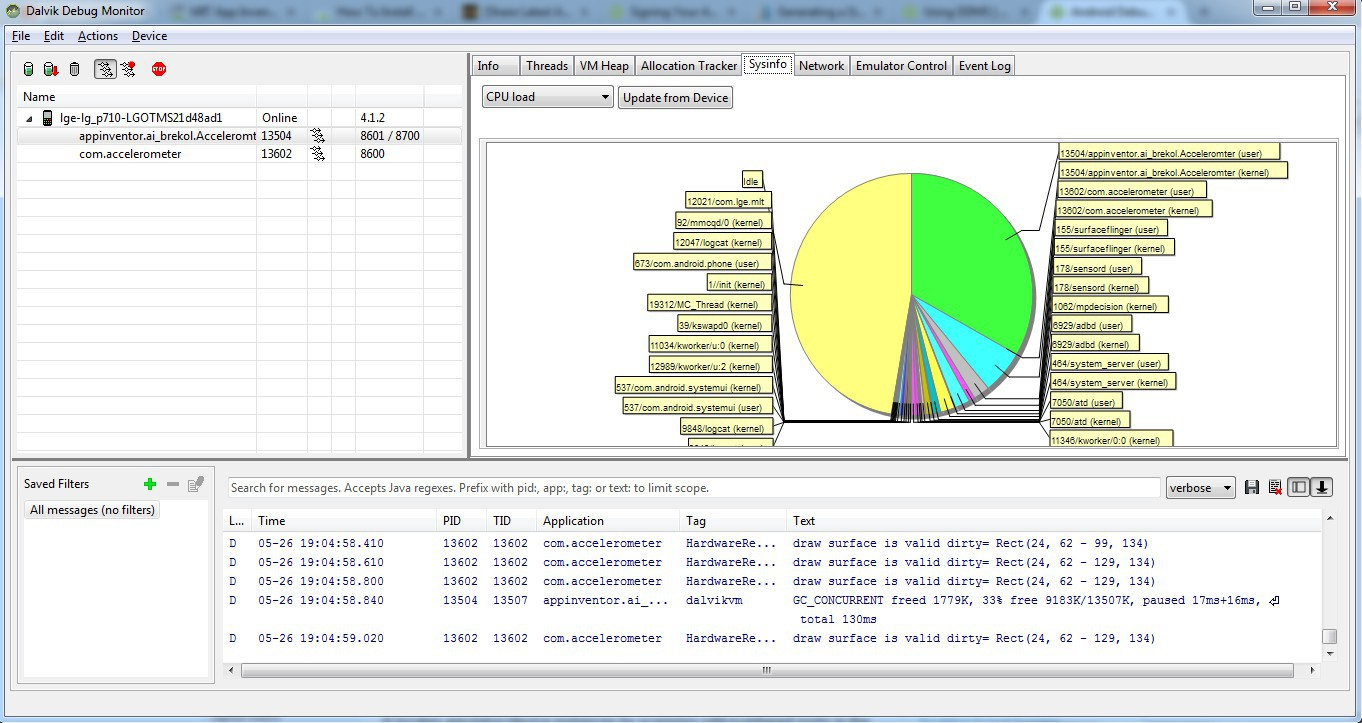
\includegraphics[width=12cm]{figures/dalvik}
\caption{Przykładowy zrzut ekranu DDMS}
\end{figure}

\section{Zużycie procesora i pamięci}

Każda aplikacja powoduje zużycie procesora oraz zajmuje miejsce w pamięci. Do pomiaru tych wielkości użyto Dalvik Debug Monitor.

Aplikację napisaną w Javie możemy konfigurować dowolnie. Między innymi, ustawiając parametr, mamy możliwość debugowania: 

\begin{lstlisting}
android:debbugable="true"
\end{lstlisting}

Jest to ważne, ponieważ aplikacja (plik *.apk) wyeksportowana z App Inventora jest niemożliwa do debugowania. Powyższy parametr ma fałszywą wartość logiczną. Aby to zmienić trzeba aplikację zdekompilować, aby zobaczyć źródła aplikacji i zmienić opcję debugowania. Dekompilacja odbywa się za pomocą darmowego narzędzia apktool.

\begin{lstlisting}
apktool -d aplikacja.apk
\end{lstlisting}

Po wykonaniu powyższej komendy zostaje tworzony folder z taką samą nazwą jak nazwa aplikacji. Plik AndroidManifest.xml jest już czytelny i możemy zmienić w nim parametr odpowiadający za debugowanie. Po zmianie, aplikację trzeba skompilować ponownie. Trzeba uruchomić poniższą komendę:

\begin{lstlisting}
apktool -b aplikacja
\end{lstlisting}

Aplikacja została skompilowana ponownie do pliku *.apk. Aby zainstalować ją na urządzeniu należy ją jeszcze cyfrowo podpisać. Generujemy klucz dla aplikacji:

\begin{lstlisting}
keytool -genkey -v -keystore keystore -alias alias_aplikacji -keyalg RSA 
-keysize 2048 -validity 20000
\end{lstlisting}

Następnie podpisujemy aplikację:

\begin{lstlisting}
jarsigner -verbose -keystore keystore aplikacja.apk alias_aplikacji
\end{lstlisting}

Ostatecznym krokiem jest zainstalowanie aplikacji na telefonie:

\begin{lstlisting}
adb install aplikacja.apk
\end{lstlisting}

Dzięki tym wszystkim czynnościom maszyna wirtualna uruchamiająca aplikacja uruchomiona na telefonie udostępnia na port umożliwiający debugowanie. Do tego portu podłącza się Dalvik Debug Monitor, z którego możemy odczytać różne statystyki aplikacji i porównać je ze statystykami aplikacji napisanej natywnie w języku Java.

\chapter{Wyniki eksperymentu}
\label{c5}

Dany rozdział zawiera wyniki z przeprowadzonych badań oraz wnioski. Każda aplikacja, która została napisana została przestawiona i opisana z różnych perespektyw. Na końcu rozdziału zostały przedstawione wady i zalety obu podejść.

\section{Stworzone aplikacje}

Aplikacje zostały najpierw stworzone w App Inventorze, a następnie zostały przepisane na język Java.

\subsection{Sortowanie}

Aplikacja polega na wygenerowaniu listy losowych elementów, a następnie posortowaniu jej. Do sortowania został użyty prosty algorytm sortowania przez wybieranie \english{Selection Sort}.

\begin{figure}[th] 
\centering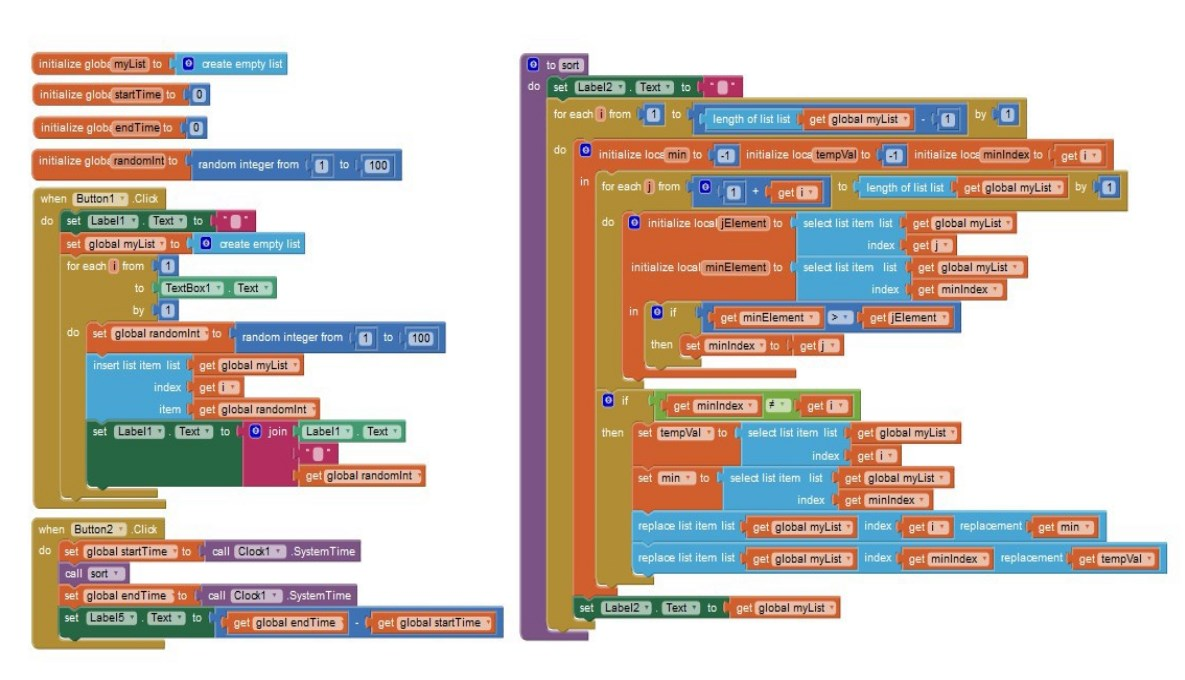
\includegraphics[width=15cm]{figures/apps/sort}
\caption{Aplikacja sortująca - App Inventor}
\end{figure}

Na powyższym rysunku widać bloki potrzebne do stowrzenia aplikacji w App Inventorze. Bez głębszej analizy zrozumienie działania bloków, może okazać się kłopotliwe. Jest to prosty algorytm, a napisanie go za pomocą dostępnych bloków okazało się skomplikowane. Można sobie łatwo wyobrazić, że napisanie bardziej skomplikowanego algorytmu byłoby bardzo nieczytelne. Ilość użytych bloków zdecydowanieby wzrosła, dodatkowo utrzymanie takiej aplikacji niesie za sobą wysokie koszty wprowadzenia nowych osób do jej rozwijania.

Sortowanie napisanie w javie jest zrozumiałe dla każdego programisty. Do sortowania została użyta lista, jako odpowiednik listy w App Inventorze, nie ma tam dostępnych tablic.


\begin{lstlisting}
 void sort(List<Integer> list){
        for(int i =0;i<list.size()-1;i++){
            int index = i;
            for(int j=i+1;j<list.size();j++){
                if(list.get(j) < list.get(index) ){
                    index = j;
                }
            }
            if(index != i){
                int tmp = list.get(i);
                list.set(i,list.get(index));
                list.set(index,tmp);
            }
        }
    }
\end{lstlisting}

W algorytmach bardzo ważna jest wydajność. Oba algorytmy działają w ten sam sposób, jednak wydajność sortowania listy napisanej w Javie jest zdecydowanie wyższa. Można to zaobserwować na poniższym wykresie. Przesortowanie bardzo małej liczby elementów zajmuje App Inventorowi bardzo dużo czasu. Przy 25 elementach czas sortowania przekroczył 1 sekundę. Jest to bardzo słaby wynik w porównaniu do sortowania napisanego w Javie. Średnio czas sortowania był 2 tysiące razy mniejszy! Na danym wykresie została zastosowana skala logarytmiczna, aby zobaczyć różnicę.

\begin{figure}[htbp]
\centering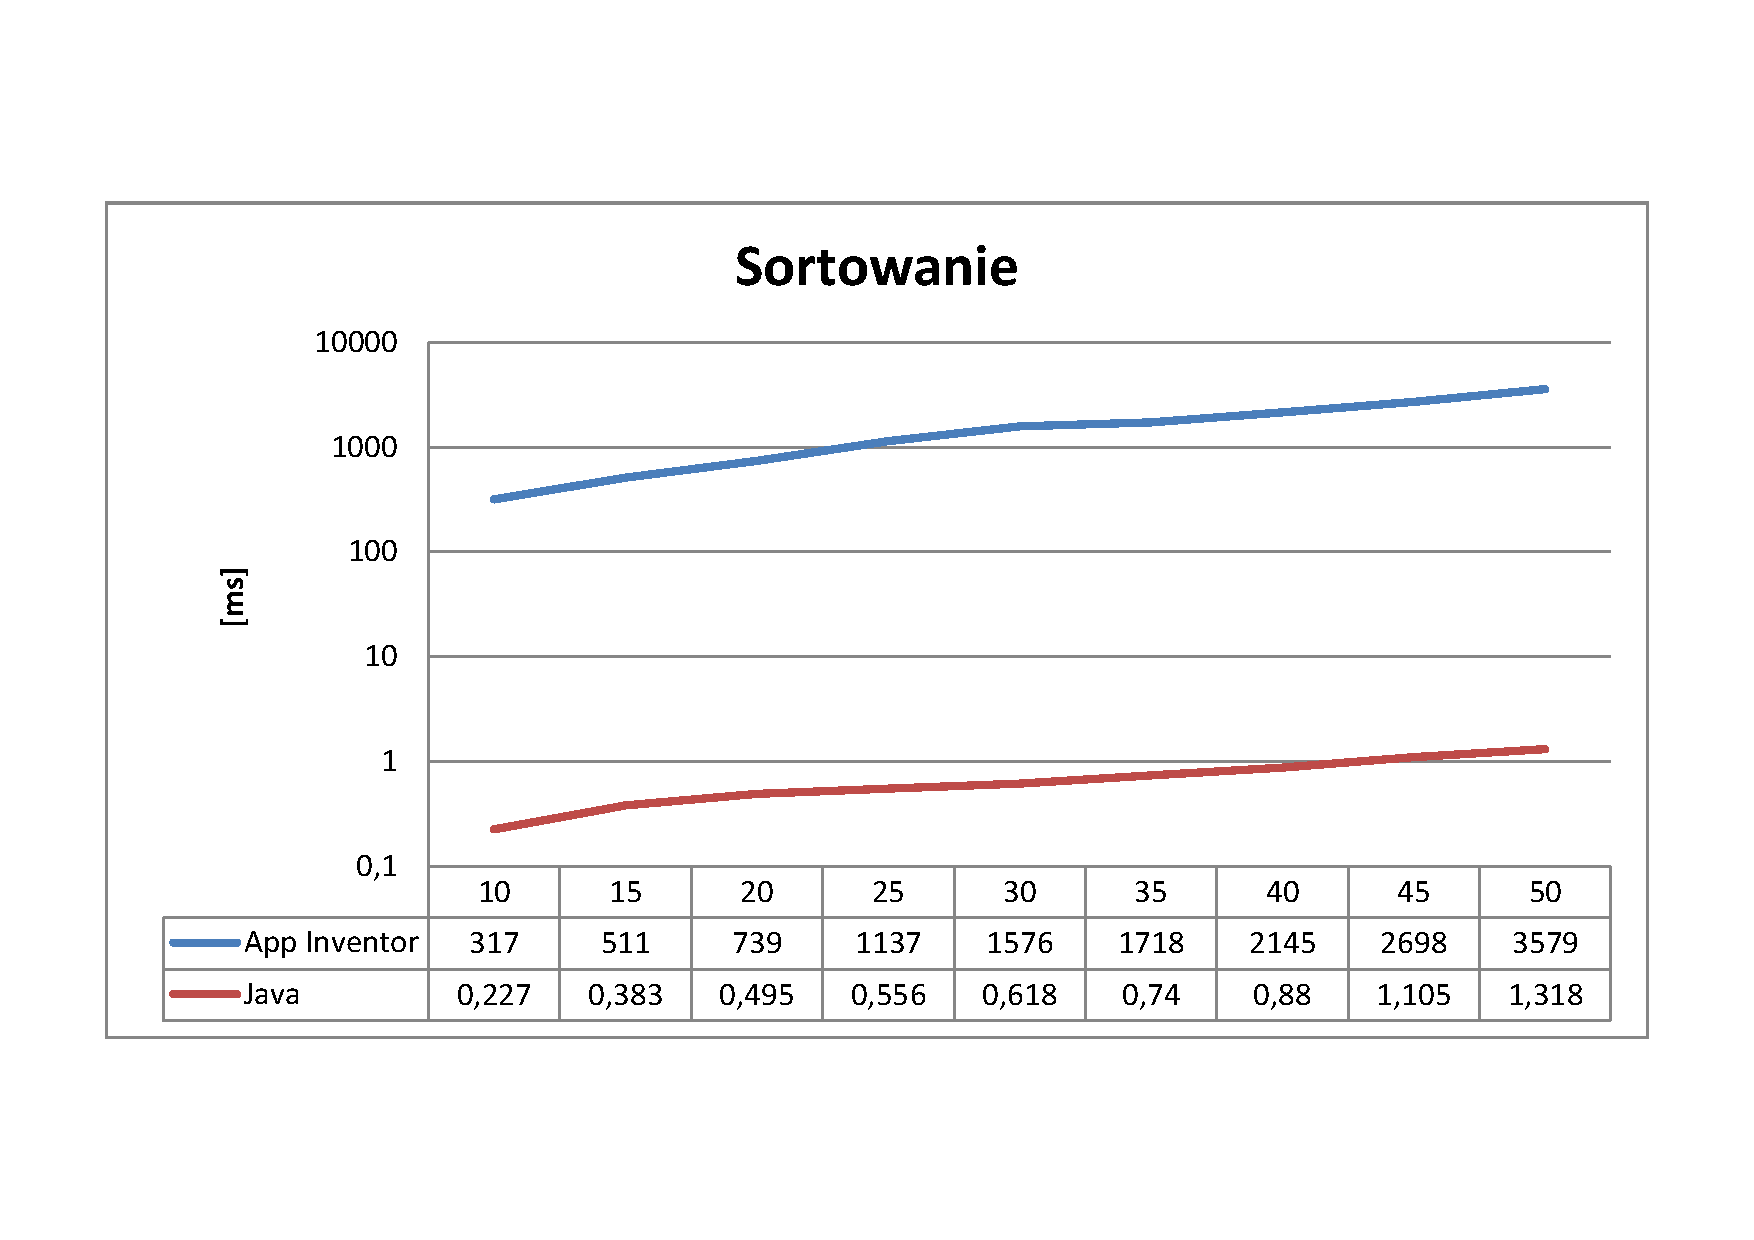
\includegraphics[width=10cm]{figures/apps/sortChart}
\caption{Wykres przedstawiający czas sortowania}
\end{figure}

Napisanie tej aplikacji w Javie nie było żadnym problemem. Bardzo łatwo było zdebugować kod i sprawdzić jego poprawność. Stworzenie tej samej aplikacji w App Inventorze nie było trywialne.


\subsection{Akcelerometr}

Kolejną aplikacją jest wykorzystująca akcelerometr. Odczytuje ona dane z akcelerometru, a następnie wyświetla je na ekran telefonu, z zadaną częstotliwością. Na poniższym wykresie przedstawione jest zużycie procesora dla różnych wartości próbkowania. Można zauważyć, że zużycie procesora dla aplikacji napisanej w Javie jest prawie stałe. Dzieje się tak dlatego że ustawianie częstotliwości próbkowania jest to tylko wskazówką dla systemu. Zdarzenia mogą być odbierane szybciej lub wolniej niż zadana częstotliwość. Zazwyczaj są odbierane szybciej. W tym przypadku są odbierane szybciej i zmiana częstotliwości na mniejszą, tak naprawdę nic tutaj nie zmienia, ponieważ zdarzenia dalej będą odbierane szybciej. Zużycie procesora prawdopodobnie będzie dalej stałe, gdy będziemy zmniejszać częstotliwość.\cite{doc:android}

\begin{figure}[H]
\centering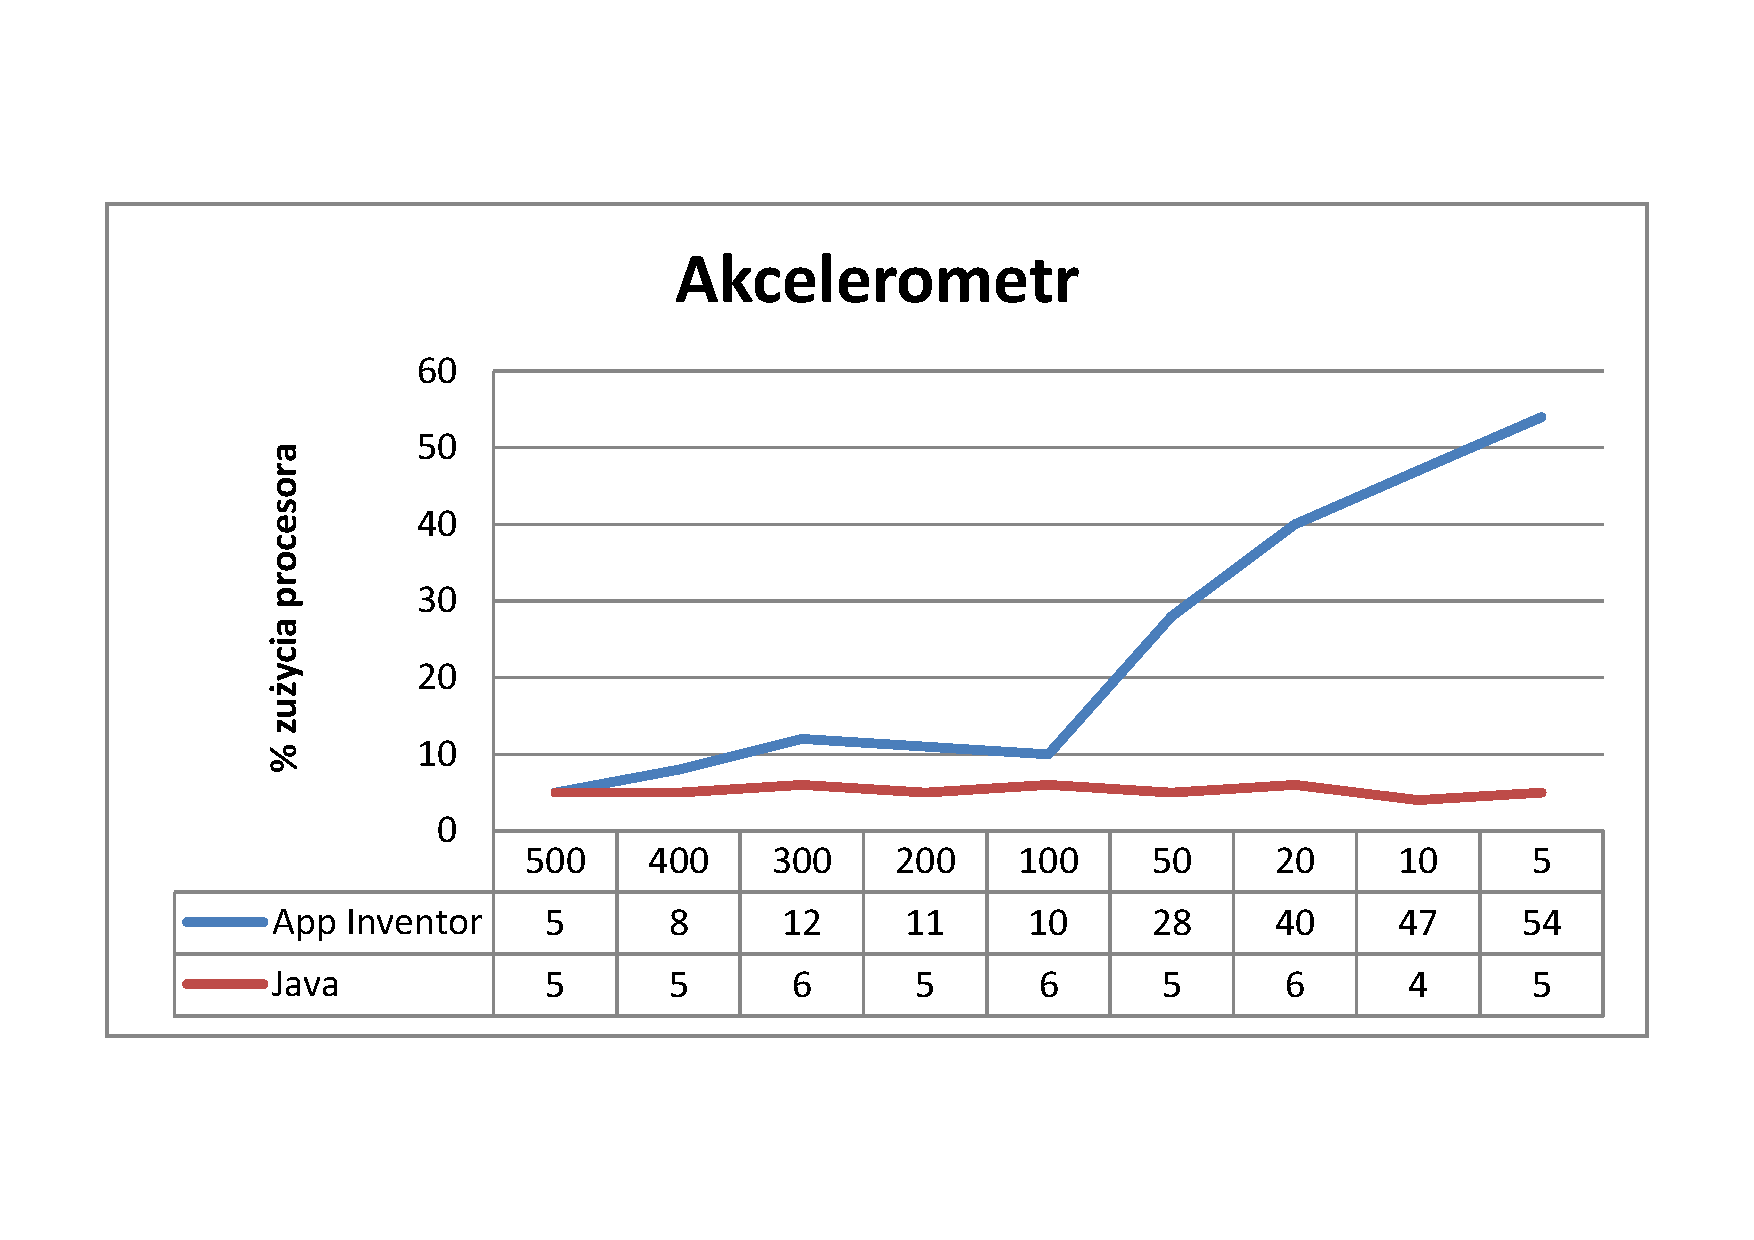
\includegraphics[width=10cm]{figures/apps/accelerometerChart}
\caption{Wykres przedstawiający zużycie procesora}
\end{figure}

W AppInventorze nie można zadać bezpośrednio akcelerometrowi częstotliwości próbkowania. Aby to obejść, trzeba dodać nowy komponent Clock, który ma możliwość uruchamiania, co zadany czas. Można podejżewać, że wydajność akcelerometru jest niezmienna i częstotliwość próbkowania jest stała. Wyraźny spadek wydajności jest przez to, że musimy wywoływać metody w bardzo krótkich odstępach czasu i to, że one dodatkowo odczytują wartość sensora, nie wpływa znacząco na zużycie procesora.


\subsection{Fibonacci}

Następną stworzoną aplikacją jest aplikacja wyliczająca kolejny element ciągu Fibonnaciego. Testuje ona wydajność App Inventora. Złożoność takiego algorytmu to $O(2^n)$, czyli czas wykonywania będzie rósł bardzo szybko. Dodatkowo, kod jest napisany tak, aby metody wykonywały się rekurencyjnie, jednak aplikacja nie jest w stanie przetestować wielkości stosu. Dla bardzo małych liczb czas wykonywania się algorytmu jest bardzo wysoki.

\begin{figure}[H]
\centering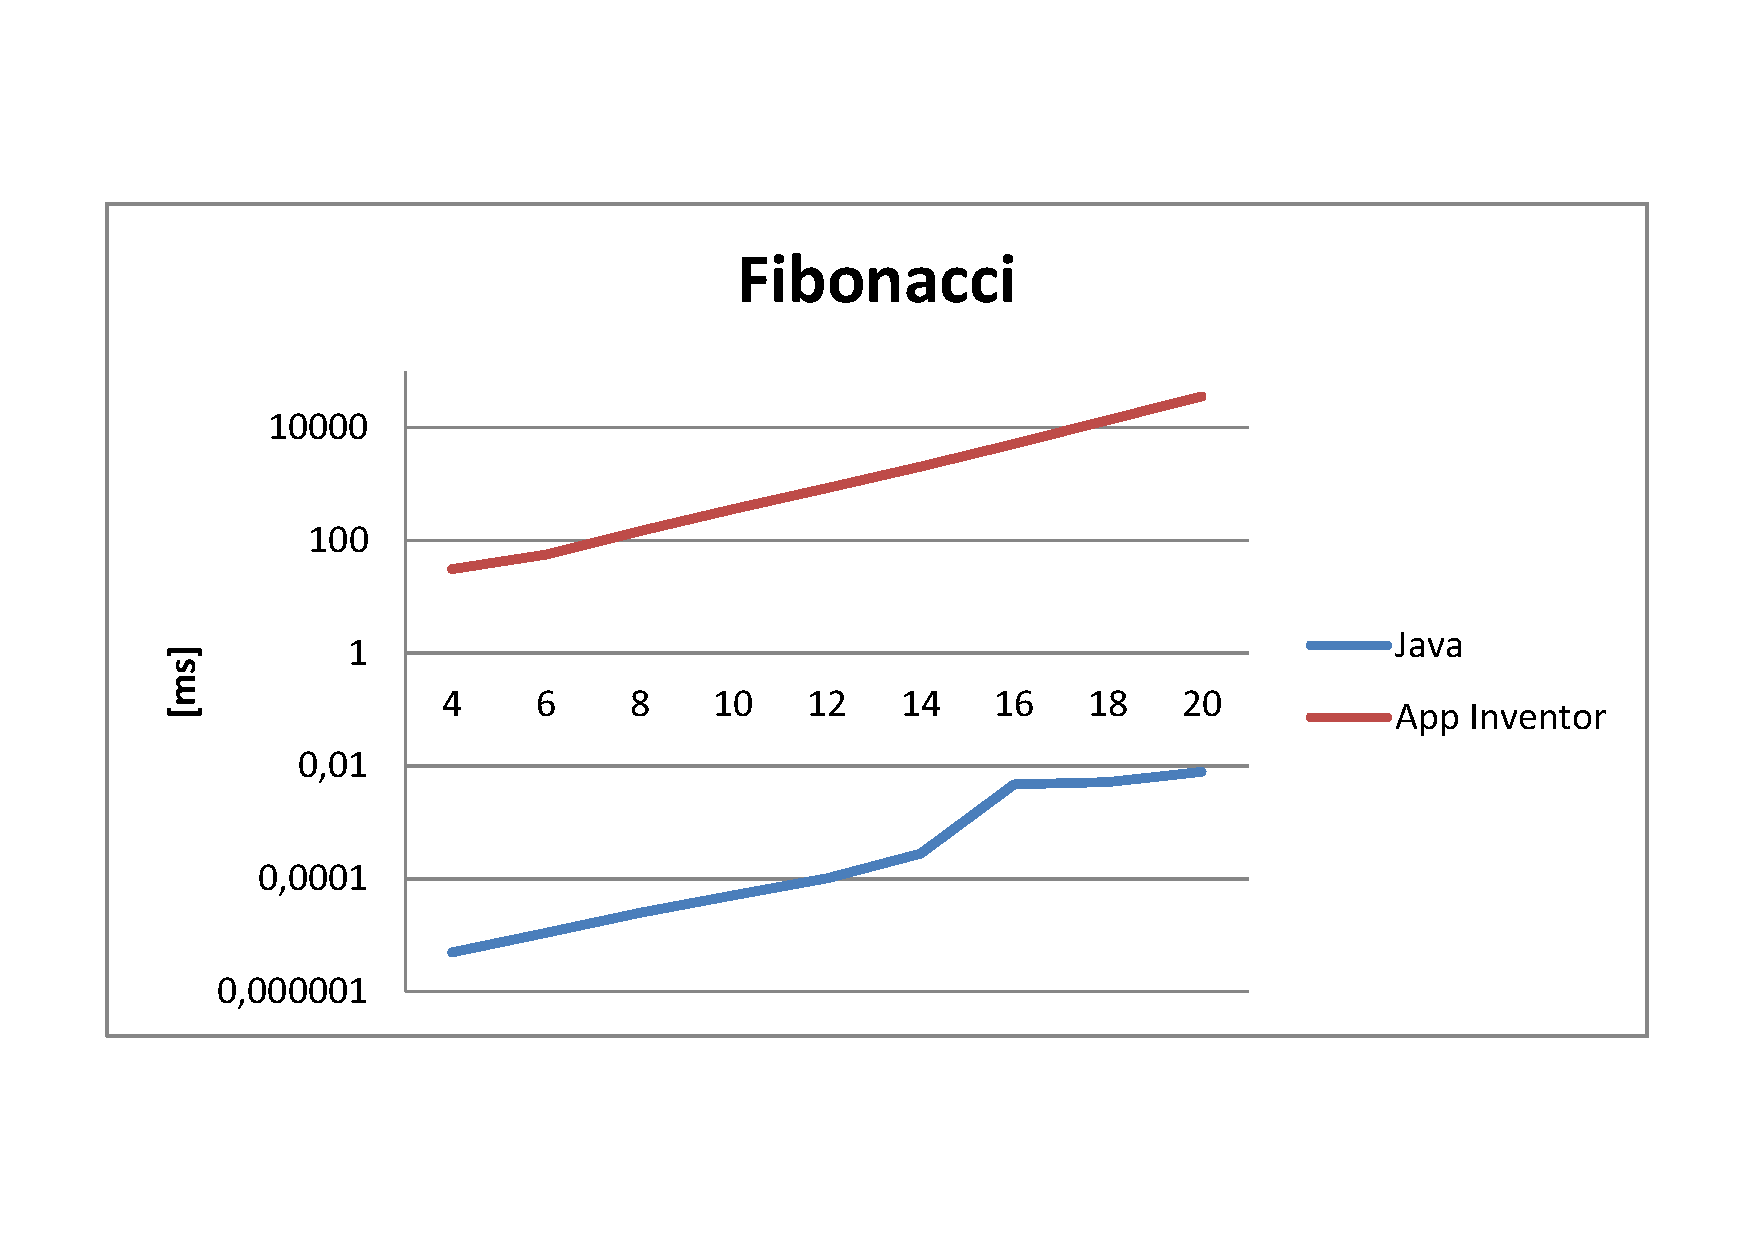
\includegraphics[width=10cm]{figures/apps/fibonacciChart}
\caption{Wykres przedstawiający czas obliczenia n-tego elementu z ciągu Fibonacciego}
\end{figure}

Osiągnięty rezultat wydajności nie jest zaskakujący po otrzymaniu wyników z poprzednich programów. Czas obliczenia już początkowych elementów ciągu Fibonnaciego jest bardzo duży. Przy liczeniu 20 elementu aplikacja napisana w App Inventorze potrzebuje ponad pół minuty, podczas gdy, aplikacja napisana w Javie potrzebuje na to około jedną setną sekundy.


\subsection{Silnia}

Następny program oblicza silnię danego elementu. Istnieje możliwość wyboru, iteracyjna lub rekursyjna wersja. Aby zaprezentować oba podejścia na jednym wykresie, została użyta skala logarytmiczna.

\begin{figure}[H]
\centering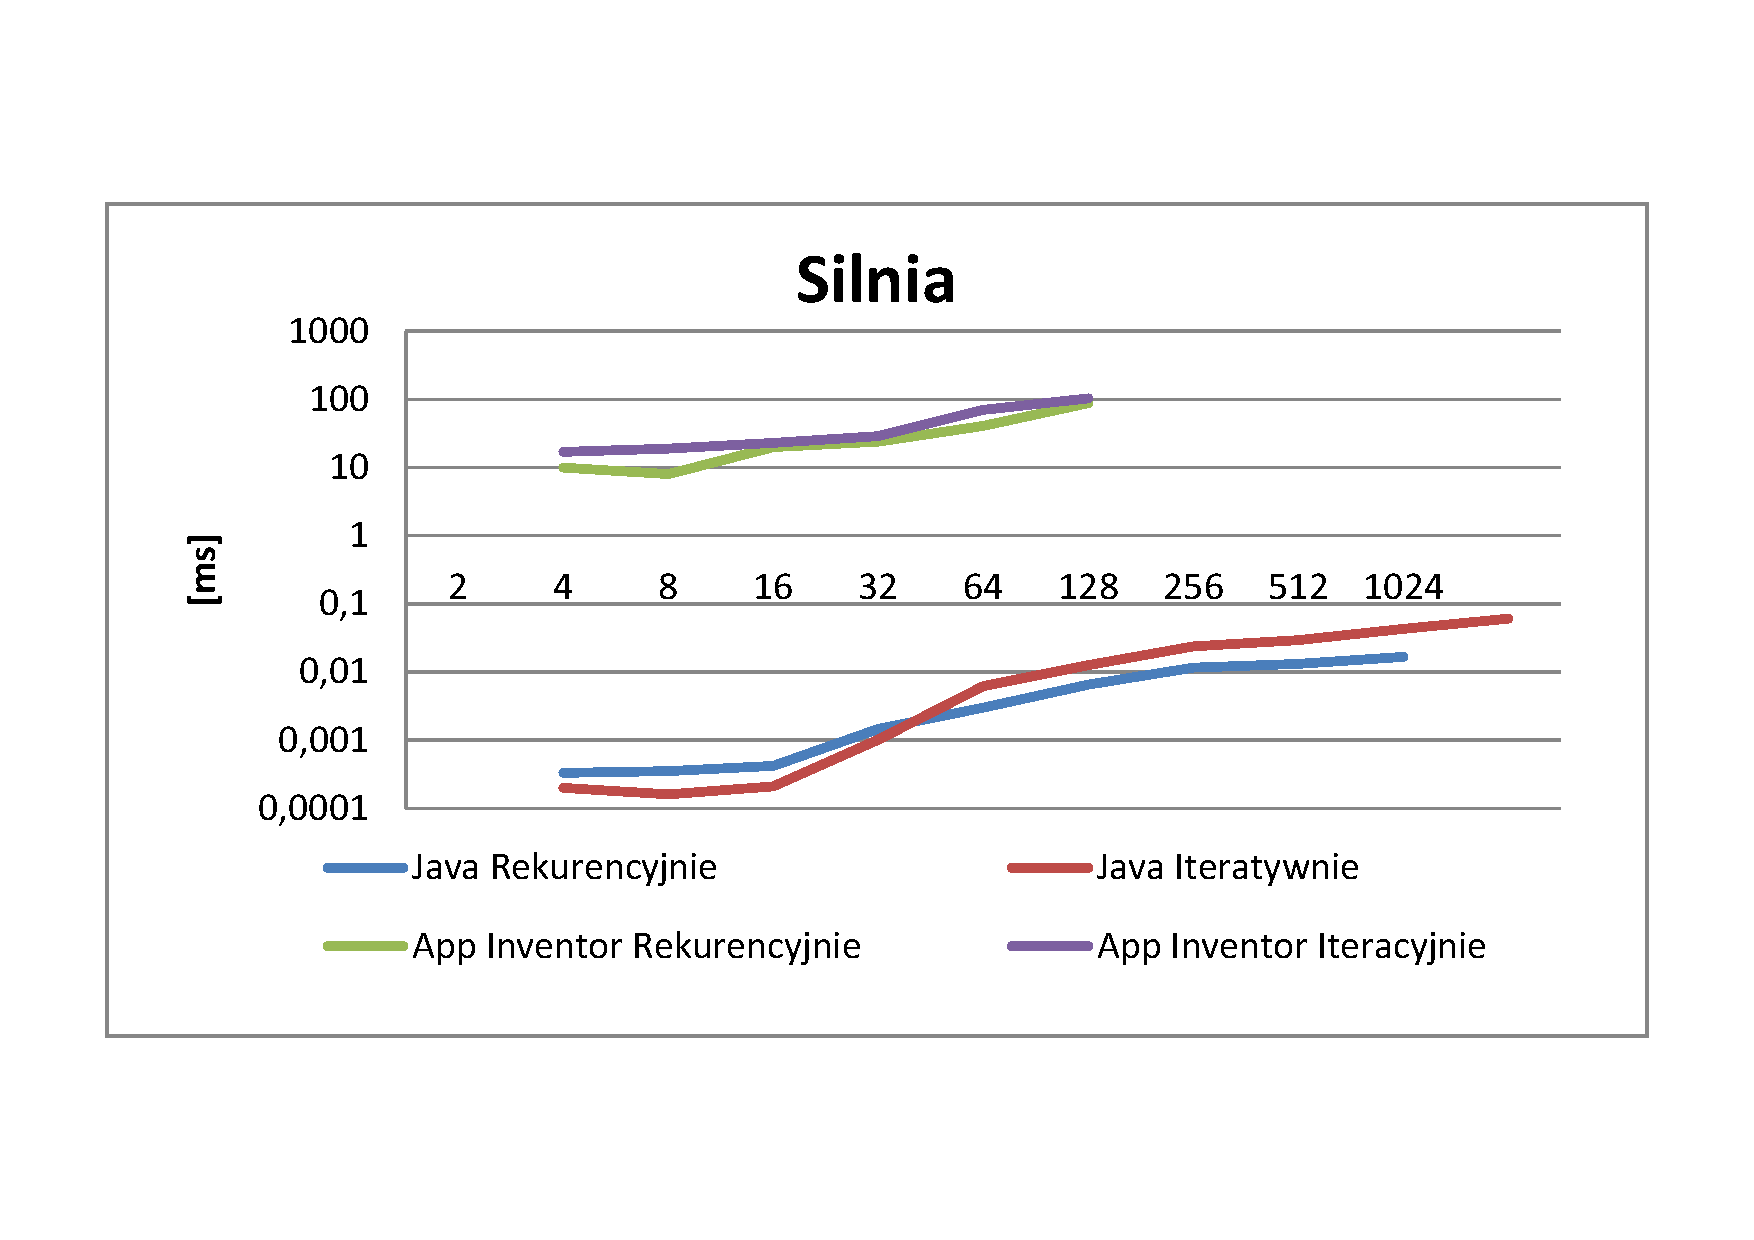
\includegraphics[width=10cm]{figures/apps/factorialChart}
\caption{Wykres przedstawiający czas obliczenia silni danego elementu}
\end{figure}

Na powyższym wykresie można zaobserować wiele istotnych elementów. Aplikacja napisana w języku Java nie miała żadnych problemów w podejściu iteracyjnym. Zakres liczb nie został przekroczony, ze względu na możliwość wyboru typu danych. Potrzebna była tutaj klasa dla wielkich liczb całkowitych, dlatego został użyty typ BigInteger. Podczas użycia wersji rekurencyjnej, przy około liczeniu silni dla około 700, program rzuca wyjątek przepełnienia stosu (\english{Stack overflow}).

Ciekawa sytuacja występuje dla aplikacji napisanej w App Inventorze. Program rzuca wyjątek podczas działania programu (\english{Runtime error}). Niestety, nie wiadomo co to za błąd, ponieważ w logach wiadomość o błędzie jest niedostępna. Wiadomość, którą otrzymujemy w logach wygląda następująco:

\begin{lstlisting}
E/com.google.appinventor.components.runtime.util.RuntimeErrorAlert:
No error message available
\end{lstlisting}

Można się jedynie domyślać, że jest to błąd przepełnienia stosu lub przekroczenia zakresu liczb.

\subsection{Database}

Aplikacja stworzona aby sprawdzić szybkość działania bazy danych oferowanej przez App Inventora. Został tutaj wykorzystany komponent TinyDB. Odpowiada on klasie Javy SharedPreferences, czyli jest to baza danych typu klucz/wartość. Aby odczytać dane z pamięci trzeba znać klucz do tych danych. Jest to bardzo łatwe w przypadku małych ilości danych, jednak trudno jest przechowywać większy struktury, ze względu na potrzebę znania klucza dla każdego wiersza. Duże ilości danych powinny być przechowywane w bazie danych SQLite, ponieważ organizacja danych i zarządzanie nimi jest wydajniejsze. Aby otrzymać część danych z bazy, trzeba posłużyć się językiem zapytań SQL. Daje to możliwość wyszukiwania interesujących nas danych. Z drugiej strony zarządzanie i przeszukiwanie dużych zbiorów danych wpływa na wydajność, więc czytanie danych z bazy danych może być wolniejsze niż czytanie danych z SharedPreferences.

\begin{figure}[H]
\centering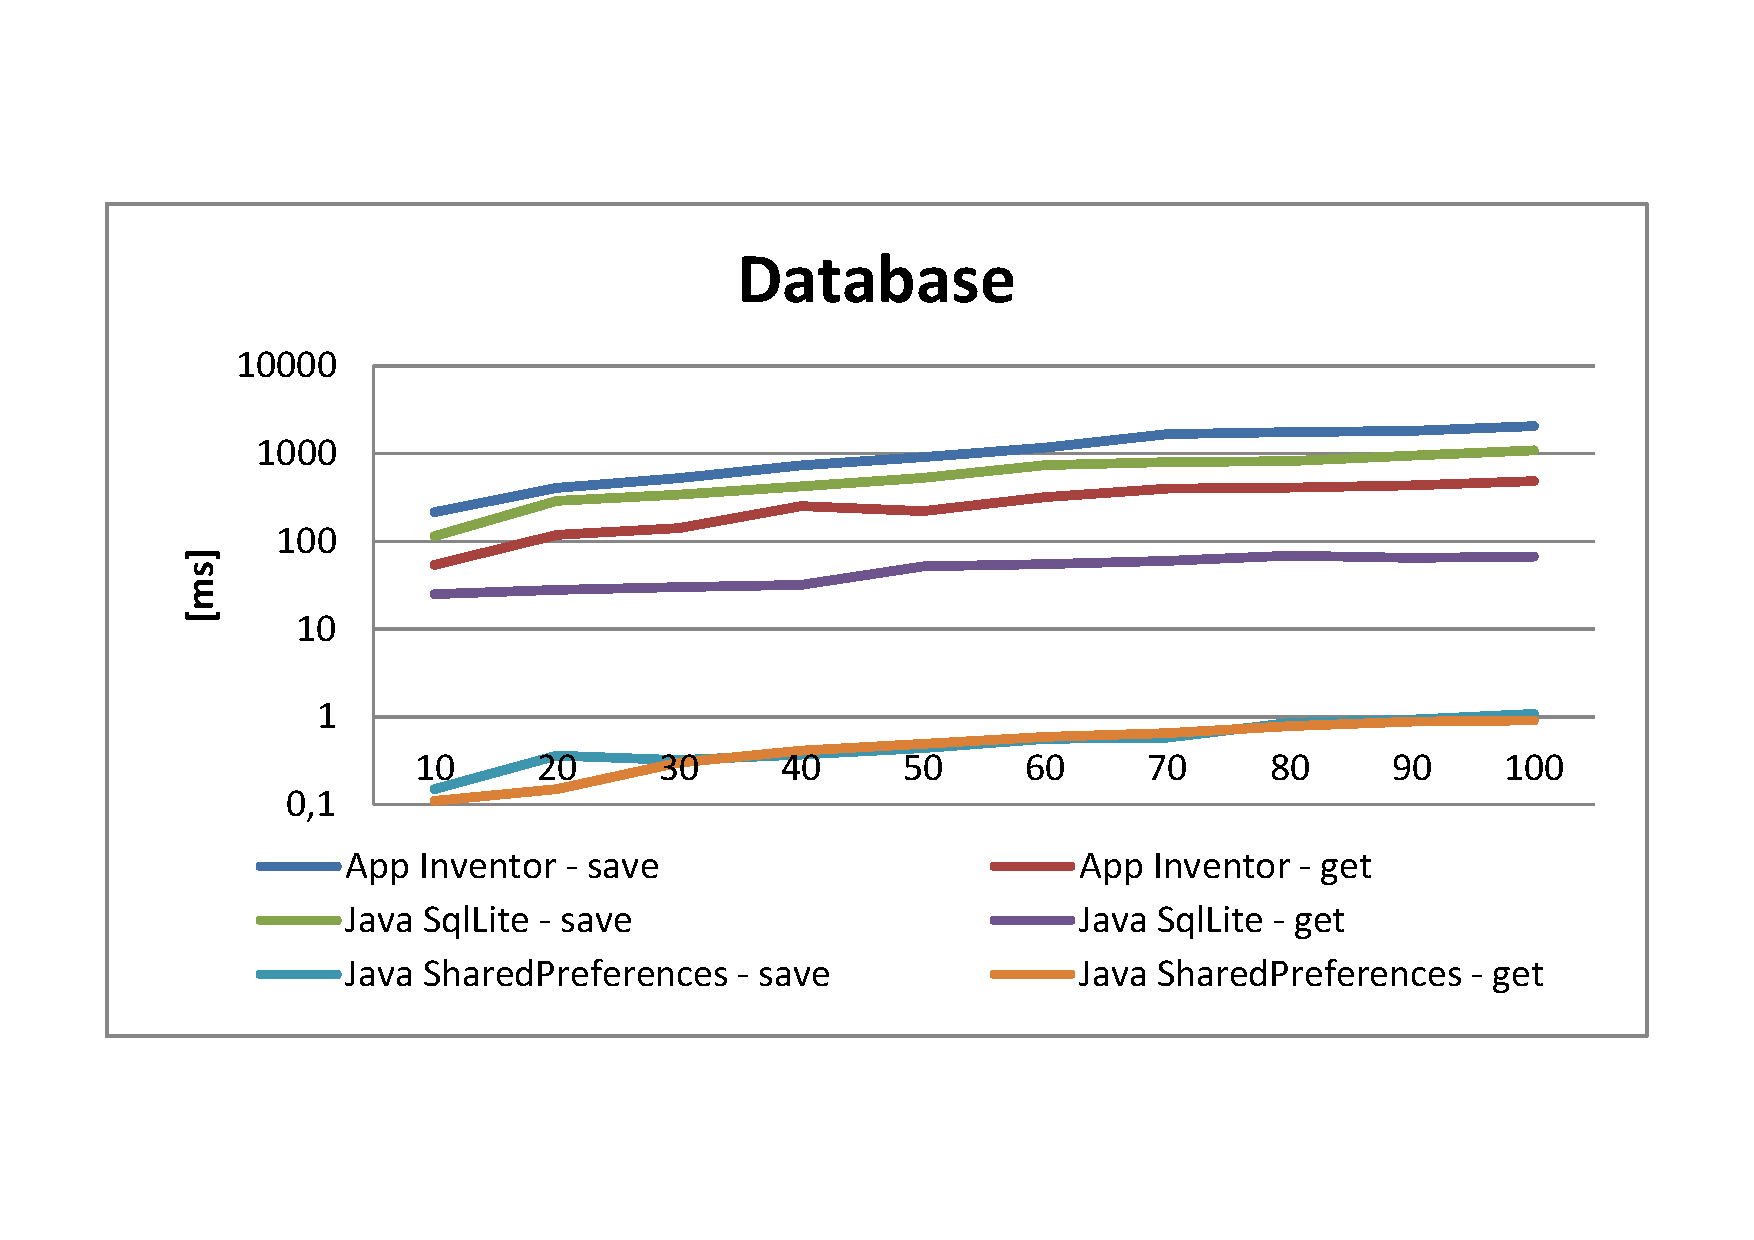
\includegraphics[width=10cm]{figures/apps/databaseChart}
\caption{Wykres przedstawiający czas potrzebny na zapis/odczyt n-elementów}
\end{figure}

Na powyższym wykresie można zauważyć przewagę wydajności aplikacji napisanej w Javie. App Inventor uzyskał podobny rezultat wydajności, jak aplikacja napisana w Javie, która używa bazy danych SQLite. Jak wspomniano wcześniej odczyt/zapis danych z bazy SQLlite powinien być wolniejszy niż korzystanie z SharedPreferences. SQLite uzykuje tutaj lepszy rezultat TinyDB - odpowiednik SharedPreferences. Można łatwo wyciągnąć wniosek, że wydajność TinyDB jest bardzo niska. Jeżeli porównamy TinyDB i SharedPreferences przewaga aplikacji napisanej w Javie jest ogromna.


\subsection{Animacja}

Aplikacja testuje możliwości animacyjne App Inventora. Wiadomo że komponenty potrzebne są dostępne, jednak nie wiadomo, czy wydajność pozwoli na płynną animację. Mimo że tworzenie animacji może wydawać się trudne, za pomocą App Inventora stworzenie animacji odbywa się tylko w kilku krokach. Największym problemem było znalezienie odpowiednich klatek, gdzie ostatnia wygląda tak samo jak pierwsza, aby była możliwość zapętlenia.


\begin{figure}[H]
\centering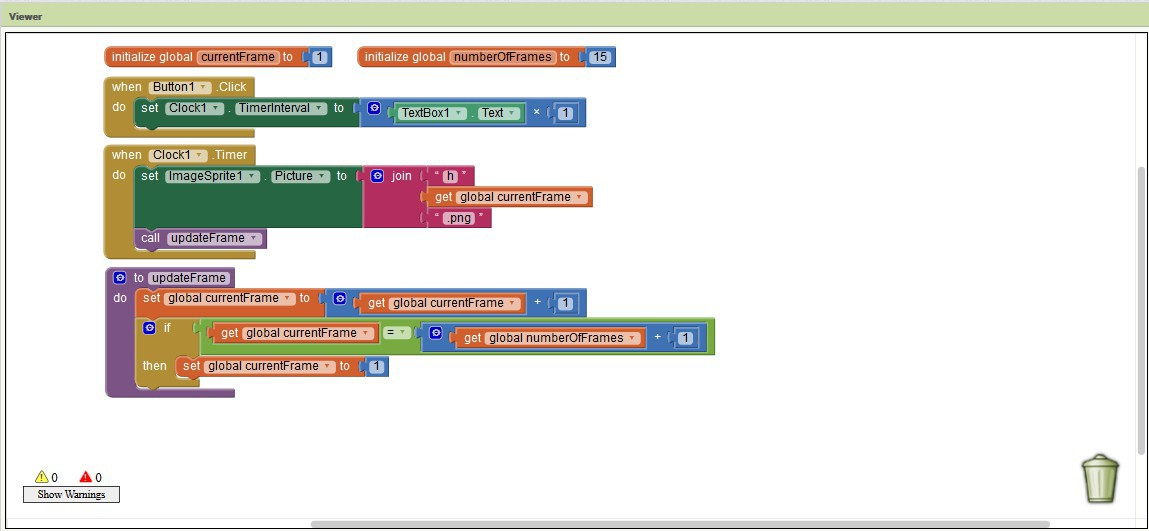
\includegraphics[width=15cm]{figures/apps/ai_animation}
\caption{Bloki potrzebne do stworzenia aplikacji}
\end{figure}

Na głównym ekranie aplikacji stworzone jest płótno oraz jeden obrazek, który podmieniamy co zadany interwał czasu. Ostatecznym rezulatatem jest płynna animacja. Dopiero przy bardzo niskim interwale czasowym (szybkiej zmianie klatek), można być odczyć przycinanie się ekranu.


\subsection{Kolizja elementów}

Aplikacja sprawdzająca możliwość detekcji kolzji poruszających się elementów. Na płótnie zostało umieszczone kilka elementów. Elementy w kolorze czarnym poruszają się po płótnie i kiedy dotrą do ściany odbijają się od niej. Element o kolorze niebieskim jest sterowanym za pomocą akcelerometru. Pochylając telefon przesuwamy element po płaszczyźnie.

\begin{figure}[H]
\centering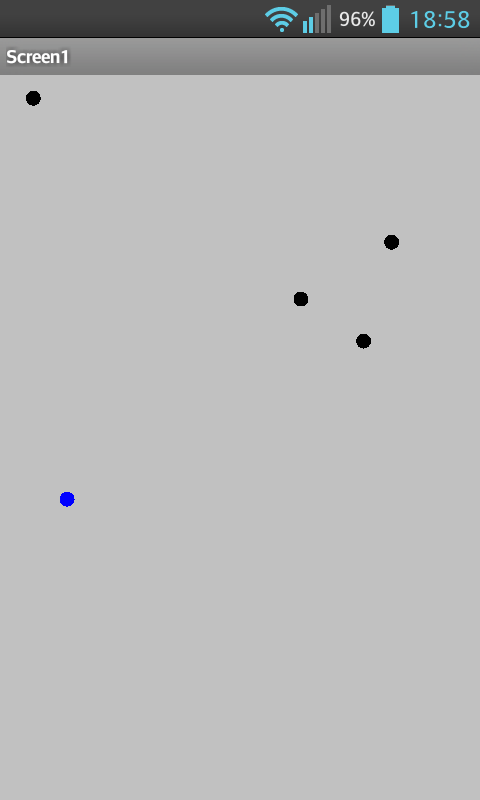
\includegraphics[width=5cm]{figures/apps/ai_collision}
\caption{Wygląd aplikacji testującec kolizje}
\end{figure}

Aplikacja działa płynnie, dla takiej ilości elementów. Wadą, którą można tutaj zauważyć, jest brak ogólnego komponentu odpowiedzialnego za zdarzenia lub możliwość przekazania parametru do zdarzenia. Jak widać na poniższym obrazku, tyle ile mamy komponentów, tyle musimy stworzyć zdarzeń odpowiedzialnych za odbicie od ściany. W danym przypadku nie jest to większym problemem. Ale kiedy istnieje potrzeba stworzenia aplikacji, która ma tych komponentów znaczącą ilość, jedną opcją jest wyklikanie zdarzeń po kolei dla wszystkich elementów.


\begin{figure}[H]
\centering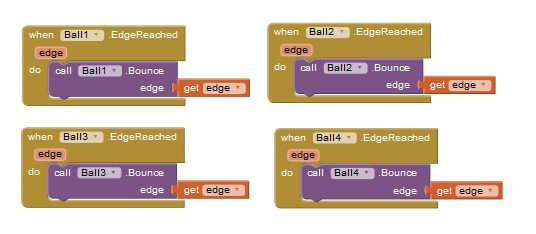
\includegraphics[width=10cm]{figures/apps/ai_collision_blocks}
\caption{Bloki odpowiedzialne za zdarzenia kolizji ze ścianą}
\end{figure}

\subsection{Activity Starter}

Aplikacja daje możliwość wystartowania nowego Activity, w App Inventor istnieje sposobność stworzenia jednej aplikacji, która będzie uruchamiała pozostałe. Odpowiedzialny za to jest komponent ActivityStarter. Wystarczy ustawić mu 2 właściwości, nazwę pakietu oraz klasy. Jeżeli w dokumentacji aplikacji nie jest napisane jakie są powyższe nazwy, warto uruchomić aplikację z podłączonym urządzeniem do komputera, aby widzieć logi. Trzeba znaleźć wtedy linijkę podobną do poniższej

\begin{lstlisting}
I/ActivityManager:
START {act=android.intent.action.MAIN cat=[android.intent.category.LAUNCHER]
flg=0x10200000 cmp=org.mozilla.firefox/.App u=0} from pid 726
\end{lstlisting}

Jeżeli pojawi się fragmet z parametrem cmp, to nazwą pakietu jest tekst przez ukośnikiem, a nazwą klasy jest cały tekst bez ukośnika. Zatem komponent ActivityStarter daje możliwość uruchomienia prawie każdej aplikacji. Aplikacja nie musi być stworzona w App Inventorze, może to być dowolna aplikacja zainstalowana na urządzeniu. Istnieje również możliwość przekazania dodatkowych parametrów, przy uruchamianiu zewnętrznej aplikacji. Niektóre z nich są nawet zaprojektowane w ten sposób, aby przyjmować dodatkowe parametry podczas uruchamiania. Przykładem są tutaj aplikacja map, która przyjmie jako paramter wartości geograficzne. Innym przykładem jest wyszukiwarka internetowa, która przyjmie jako parametr tekst do wyszukania lub adres do wyświetlenia.

\begin{lstlisting}
Action: android.intent.action.VIEW
DataUri: http://google.pl
\end{lstlisting}

Ustawiając powyższe parametry, uruchomi się przeglądarka internetowa na stronie http://google.pl. Druga możliwość jaką daje ActivityStarter to odbieranie parametrów. W App Inventorze istnieje tylko przekazywanie wartości tekstowych. Aby zwrócić taki parametr trzeba użyć bloku zamykającego aplikację z właściwością do ustawienia (\english{Close Application With Plain Text}).

\subsection{Multiple Screens}

Jeżeli obie aplikacje mają być napisane przez tego samego programistę, warto się zastanowić, czy nie zrobić jednej aplikacji z wieloma ekranami. Zwiększy to użyteczność aplikacji, użytkownicy nie będą musieli instalować dwóch. Używając ActivityStartera dotychczas istnieje możliwość przekazywania tylko parametrów tekstowych. Natomiast przy użyciu wielu ekranów, można przekazywać dodatkowo listy. Kiedy aplikacja korzysta z bazy danych, również jest ona współdzielona pomiędzy ekranami. Otworzony ekran daje możliwość powrotu do ekranu, który go otworzył. Ilość ekranów nie jest ogarniczona, ale zamknięcie ekranu powraca do tego, który go otworzył. Z drugiej strony łatwo to obejść, tworząc ekran, który będzie menadżerem innych ekranów i będzie on uruchamiał pozostałe. Jeżeli z uruchomionego ekranu użytkownik będzie chciał przejść do innego, aplikacja powróci do menadżera z parametrem, a menadżer w odpowiedzi na dany paramter otworzy inny ekran. Zatem tak samo jak w przypadku aplikacji wykorzystującej komponent ActivityStarter istnieje możliwość przekazywania i odbierania parametrów pomiędzy ekranami. Każdy stworzony ekran będzie miał swój wygląd oraz własne komponenty w oknie Designera. Stworzenie jednej bazy danych może być trochę nieintuicyjnie, ponieważ każdy ekran musi posiadać swój komponent TinyDB. Aczkolwiek jest to jedna i ta sama baza danych. Jeżeli jeden ekran zapisze jakąś wartość, drugi może ją odrazu odczytać.




\section{Zalety programowania wizualnego}

\section{Wady programowania wizualnego}

Przynajmniej na razie nie ma możliwości rozszerzenia App Inventora, więc jeżeli istniałaby potrzeba stworzenia lub skorzystania z czegoś, co nie jest wbudowane bezpośrednio w oferowaną platformę, jak np. grafika 3D, to ostatecznie okaże się że projekt nie zostanie zrealizowany.

Implementacja App Inventora nie jest zoptymalizowana dla gier o wysokiej wydajności.

\chapter{Wnioski}
\label{c6}

\section{Zalety programowania wizualnego}

Główną zaletą programowania wizualnego jest łatwość, z jaką przychodzi pisać aplikacje. Nie trzeba być doświadczonym programistą, aby tworzyć aplikacje za pomocą App Inventora. Jeżeli ktoś jest zainteresowany programowaniem i nie wie jak zacząć, programowanie wizualne może okazać się dobrym wyborem na start. Nauka programowania wizualnego nie jest skomplikowana, wystarczą chęci. 

Kolejną zaletą jest nieskomplikowany sposób stworzenia dobrze wyglądającego interfejsu graficznego (\english{GUI}). Nie znać języku XML aby zdefiniować ładny układ i wygląd ekranu. Wszystkie elementy są przeciągane z palety komponentów, a ich właściwości ustawiane również w prosty sposób.

Następną zaletą są możliwości jakie daje programowanie wizualne. Mimo, że wiele funkcji nie jest dostępnych to aplikacje, które można stworzyć za pomocą App Inventora mogą być bardzo rozbudowane. Komponenty oferowane przez to środowisko pokrywają zdecydowaną większość podstawowych i najbardziej używanych elementów, których się używa podczas pisania aplikacji w języku Java. Jeżeli jakiegoś komponentu brakuje, np. przycisków typu Radio, w internecie jest wiele materiałów w jaki sposób można to obejść.

Myślenie wizualne jest bardziej naturalne dla człowieka. Programowanie w App Inventorze daje programistom możliwość pisania programów poprzez manipulację elementami graficznymi. Dopiero doświadczony programista będzie potrafił sobie wyobrazić na wyższym poziomie abstrakcji kod tekstowy. Dlatego też kod aplikacji Javowej musi spełniać założenia wzorców projektowych, dzięki czemu łatwość nawigowania pomiędzy klasami i metodami jest dużo większa. W App Inventorze stworzenie zadanej funkcjonalności sprowadza się zwykle do użycia pojedynczych bloków, co daje dużą przejrzystość. Dopiero skomplikowane aplkiacje mogłyby rozrosnąć się, tak że zrozumienie ich zajełoby dużo więcej czasu niż takiej samej aplikacji napisanej w języku Java. Jednak jeżeli jest to tak skompilkowana aplikacja warto się zastanowić czy napisanie jej w App Inventorze to dobry pomysł.

App Inventor może być również dobrym narzędziem do tworzenia prototypów. Aplikacje tworzone za pomocą niego powstają bardzo szybko. Stworzony układ graficzny można w krótkim czasie zaprezentować biznesowi, który dzięki temu będzie miał szansę szybko zareagować i skorygować lub zatwierdzić dany interfejs.

\section{Wady programowania wizualnego}

Przynajmniej na razie nie ma możliwości rozszerzenia App Inventora, więc jeżeli istniałaby potrzeba stworzenia lub skorzystania z czegoś, co nie jest wbudowane bezpośrednio w oferowaną platformę, jak np. grafika 3D, to ostatecznie okaże się że projekt nie zostanie zrealizowany.

Implementacja App Inventora nie jest zoptymalizowana dla gier o wysokiej wydajności. Cały framework App Inventora zużywa o wiele więcej mocy procesora, niż programy napisane w języku Java. Przy zwykłym sortowaniu program napisany w Javie jest średnio 2 tysiące razy szybszy.

Stworzenie większego projektu i decyzja o użyciu App Inventora pociąga za sobą zaangażowanie wielu programistów. Nie mogą oni jednak pracować współbieżnie. Współdzielenie projektu odbywa się na zasadzie wyeksportowania go na komputer jako spakowane archiwum. Następnie kolejny programista może go zaimportować. Nie ma to jednak większego sensu, ponieważ kiedy dwie osoby będą pracować nad tym samym projektem, nie będzie można go na końcu scalić. Odwrotnie jest przy pisaniu aplikacji w języku natywnym. Istnieje bardzo wiele narzędzi do rozwiązania tego problemu, są to tzw. systemy zarządzania wersją kodu (\english{Source code management systems}).

\section{Inne ograniczenia App Inventora}

\begin{itemize}
\item Animacja nie jest wspierana automatycznie. Jeżeli programista chciałby stworzyć animowany GIF, posiadając kilka różnych obrazków, z których ten GIF miałby się składać, musi zrobić to manualnie. Zautomatyzowanie tego procesu byłoby bardzo pomocne.\cite{android:57}
\item App Inventor nie wspiera gestów multi-touch, czyli dotykania ekranu i wykonywanie czynności kilkoma palacmi w jednym momencie.\cite{android:57}
\item Brak wsparcia dla rysowania obrazków o standardowych kształtach. Są to między innymi prostokąty, trójkąty, koła, tekst. Programista chcąc dodać nowy element musi najpierw go stworzyć ręcznie a następnie wysłać na serwer App Inventora.\cite{android:57}
\item Niemożliwe jest tworzenie widżetów. App Inventor nie wspiera danej funkcji
\end{itemize}



% All appendices and extra material, if you have any.
\cleardoublepage\appendix%
\chapter{Content of the DVD}

As an addition to this document, the DVD is attached. It provides some materials connected with the presented subject in electronic form for potential users or people, who would want to continue works on this topic. 

The DVD content consists of several items:

\begin{enumerate}
\item Item 1
\item Item 2
\item Item 3
\end{enumerate}



% Bibliography (books, articles) starts here.
\bibliographystyle{alpha}{\raggedright\sloppy\small\bibliography{bibliography}}

% Colophon is a place where you should let others know about copyrights etc.
\ppcolophon

\end{document}
